\documentclass[a4paper, 12pt]{article}
\usepackage[utf8x]{inputenc}
\usepackage{cmap}
\usepackage[english, russian]{babel}
\usepackage{indentfirst}
\usepackage[left=20mm, top=20mm, right=20mm, bottom=20mm]{geometry}
\usepackage{tikz}
\usepackage{amsmath, amsfonts, amssymb}
\usepackage{graphicx}
\usepackage{fancybox, fancyhdr}
\usepackage{hyperref}
\usepackage{listings}
\usepackage{caption}
\usepackage{subcaption}
\usepackage{xcolor}
\pagestyle{fancy}
\fancyhf{}
\fancyhead[L]{Лабораторная работа №3}
\fancyhead[R]{Частотные методы}
\fancyfoot[C]{\thepage}
\graphicspath{{images/}}
\usetikzlibrary{patterns}
\definecolor{LightGray}{gray}{0.95}
\lstdefinestyle{pycode}{
    language=Python,
    basicstyle=\footnotesize\ttfamily,
    numbers=left,
    numberstyle=\tiny\color{gray},
    stepnumber=1,
    numbersep=5pt,
    backgroundcolor=\color{LightGray},
    showspaces=false,
    showstringspaces=false,
    showtabs=false,
    tabsize=4,
    captionpos=b,
    breaklines=true,
    breakatwhitespace=false,
    frame=none,
    rulecolor=\color{black},
    linewidth=\linewidth,
    keywordstyle=\color{red}\bfseries,
    commentstyle=\color{green!40!black},
    stringstyle=\color{blue},
    escapeinside={\%*}{*)},
    xleftmargin=0pt,
    framexleftmargin=0pt,
    framexrightmargin=0pt,
    inputencoding=utf8/utf8x,
    extendedchars=\true
}
\lstset{style=pycode}
\hypersetup{
    colorlinks=true,
    linkcolor=blue,
    filecolor=magenta,      
    urlcolor=cyan,
    pdftitle={contents setup},
    pdfpagemode=FullScreen,
}
\setlength{\parskip}{1.5mm}
\setlength{\headheight}{15pt}
\setlength{\footskip}{15pt}
\allowdisplaybreaks
\DeclareMathOperator{\sinc}{sinc}
\newcommand{\frc}[2]{\raisebox{2pt}{$#1$}\big/\raisebox{-3pt}{$#2$}}

\begin{document}
    \begin{titlepage}

        \begin{center}
        
\includegraphics[width=0.3\textwidth]{itmo.png} % requires itmo.png in /images folder
        \vfill
        
        Федеральное государственное автономное образовательное учреждение высшего образования
        «Национальный Исследовательский Университет ИТМО»\\
        
        \vfill
        {\large\bf ЛАБОРАТОРНАЯ РАБОТА №3}\\
        {\large\bf ПРЕДМЕТ «ЧАСТОТНЫЕ МЕТОДЫ»}\\
        {\large\bf ТЕМА «ЖЕСТКАЯ ФИЛЬТРАЦИЯ»}
        \vfill

        \begin{flushright}
            \begin{minipage}{.45\textwidth}
            {
                \hbox{Лектор: Перегудин А. А.}
                \hbox{Практик: Пашенко А. В.}
                \hbox{Студент: Румянцев А. А.}
                \hbox{Поток: ЧАСТ.МЕТ. 1.3}
                \hbox{}
                \hbox{Факультет: СУиР}
                \hbox{Группа: R3241}
            }
            \end{minipage}
        \end{flushright}
        
        \vfill
                
        Санкт-Петербург\\
        2024
        \end{center}
    \end{titlepage}
    
    \tableofcontents

    \newpage
% \end{document}
    \section{Задание 1. Жесткие фильтры.}
    Зададим такие числа $a,\,t_1,\,t_2$, что $t_1<t_2$, и рассмотрим функцию $g$ такую, что
    $g(t)=a$ при $t\in[t_1,t_2]$ и $g(t)=0$ при других $t$. $$\sqsupset a=2,\ \ t_1=-1.5,\ \ t_2=2.5,\ \ g(t)=
    \begin{cases}
        2, & t\in[t_1,t_2]\\
        0, & \text{ otherwise}
    \end{cases}
    $$


    Выберем интервал времени $T=10$ и шаг дискретизации $dt=0.1$. Зададим в python массив времени $t$ от $-0.5\cdot T$ до $0.5\cdot T+dt$
    с шагом $dt$ и включим последнюю точку. Найдем список значений $g$ и зададим зашумленную версию сигнала как
    $$
    u=g+b\cdot(\text{random}(\text{len}(t))-0.5) + c\cdot \sin(d\cdot t);
    $$


    В данном задании мы выполняем жесткую фильтрацию сигнала $u$. Алгоритм следующий: находится Фурье-образ от сигнала,
    обнуляются его значения на некоторых диапазонах частот, затем сигнал восстанавливается обратным преобразованием Фурье.
    Далее строятся графики с помощью программы на языке python. Используемый код с пояснениями находится в отдельной секции.


    В задаваемом сигнале параметр $a$ отвечает за высоту, на которую поднимется часть сигнала от нуля, а $t_1 \text{ и } t_2$ -- начало
    и конец промежутка с подъемом соответственно. Таким образом, на интервале длины $t_2-t_1=2.5+1.5=4$, начиная с $t_1=-1.5$ и заканчивая $t_2=2.5$,
    на высоте $a=2$ будет находится часть от всего сигнала, который, в свою очередь, располагается на промежутке $[-0.5\cdot T,0.5\cdot T]=[-5,5]$
    длины $2\cdot T\cdot 0.5=10$. Параметры $b,\,c,\,d$ отвечают за шум, присутствующий в сигнале. Далее будут рассмотрены графики и сделаны выводы о
    влиянии каждого параметра на сам сигнал и на его результат фильтрации.


    \subsection{Убираем высокие частоты.}
    Возьмем параметр $c=0$. Далее действуем в соответствии с алгоритмом. Возьмем некоторый диапазон частот $[-\nu_0, \nu_0]$, на котором оставим Фурье-образ
    сигнала $u$ неизменным, а на остальных частотах обнулим его значения. Построим сравнительные графики исходного и фильтрованного сигналов на некотором
    интервале $[t_1,t_2]$, а также модуля Фурье-образа исходного и фильтрованного сигналов. Исследуем влияние частоты среза $\nu_0$ и значения параметра $b$
    на эффективность фильтрации.
    
    
    Далее будут приведены рисунки полученных графиков. На каждом графике подписаны выбранные значения $b,\,c,\,d,\,\nu_0$
    (хотя, при условии, что $c=0$, менять или рассматривать параметр $d$ не требуется). Также отмечена легенда -- синим цветом
    обозначается оригинальный сигнал, красным фильтрованный.


    \begin{figure}[!htb]
        \centering
        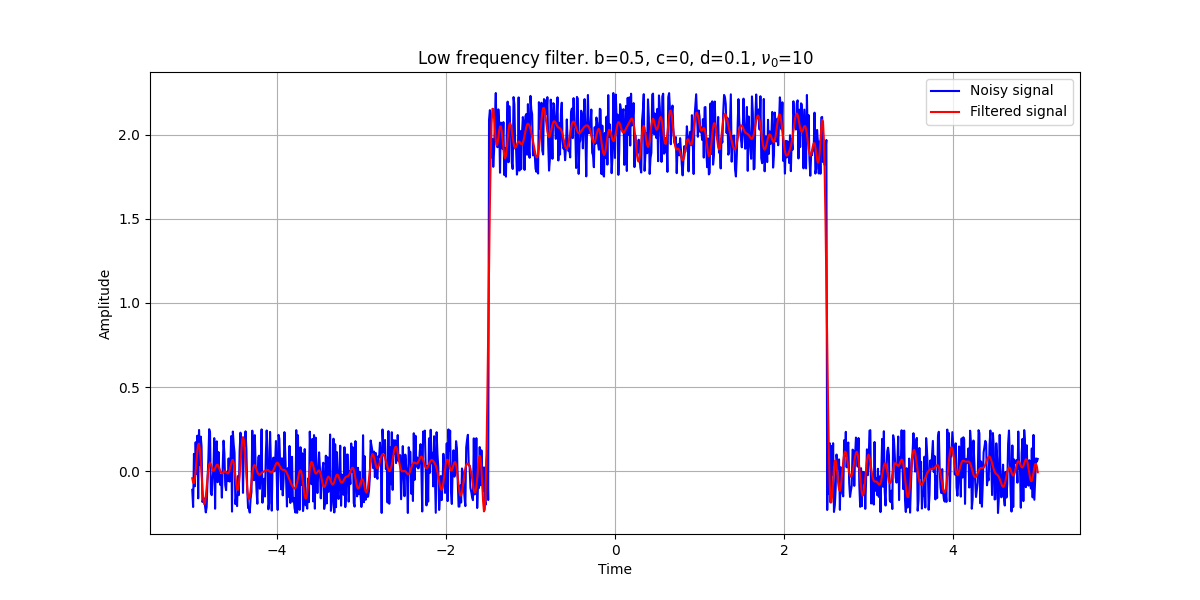
\includegraphics[scale=0.485]{1_u_flt_u_nohigh.png}
        \captionsetup{skip=0pt}
        \caption{График исходного и фильтрованного сигналов}
        \label{fig:fig1}
    \end{figure}
    \begin{figure}[!htb]
        \centering
        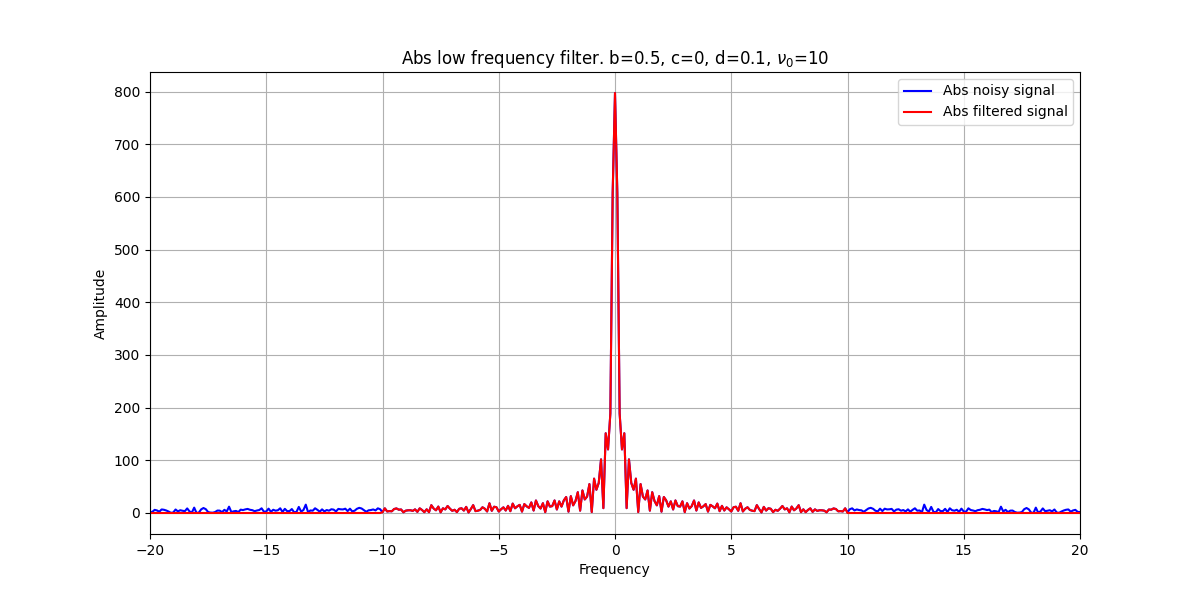
\includegraphics[scale=0.485]{1_abs_u_U_nohigh.png}
        \captionsetup{skip=0pt}
        \caption{График модуля Фурье-образа исходного и фильтрованного сигналов}
        \label{fig:fig2}
    \end{figure}
    \begin{figure}[!htb]
        \centering
        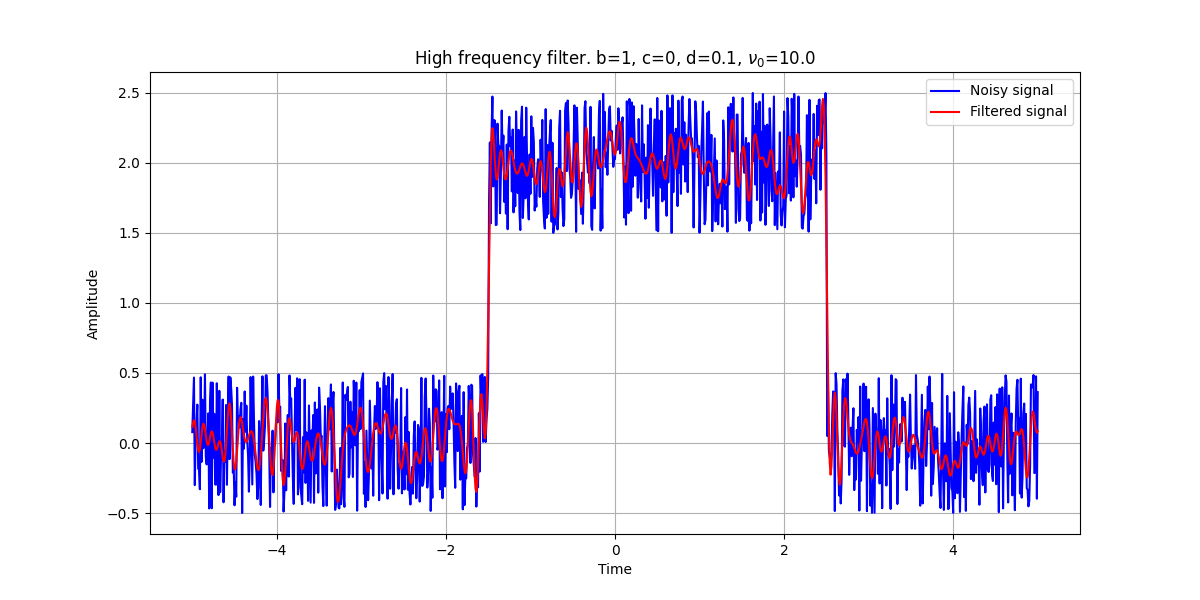
\includegraphics[scale=0.485]{2_u_flt_u_nohigh.png}
        \captionsetup{skip=0pt}
        \caption{График исходного и фильтрованного сигналов}
        \label{fig:fig3}
    \end{figure}
    \begin{figure}[!htb]
        \centering
        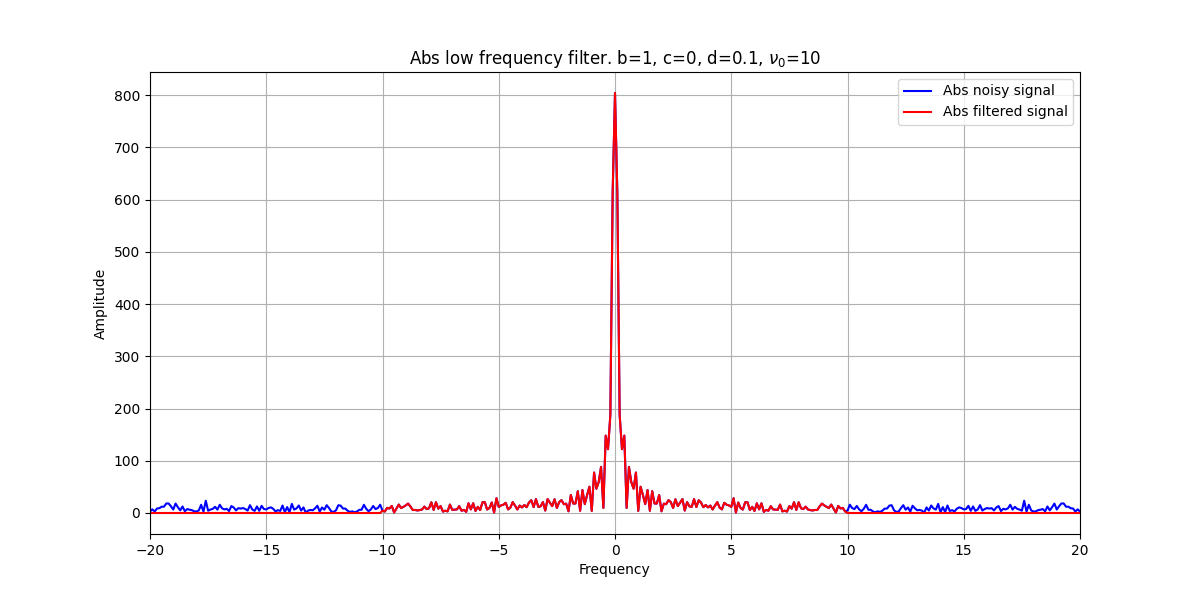
\includegraphics[scale=0.485]{2_abs_u_U_nohigh.png}
        \captionsetup{skip=0pt}
        \caption{График модуля Фурье-образа исходного и фильтрованного сигналов}
        \label{fig:fig4}
    \end{figure}
    \begin{figure}[!htb]
        \centering
        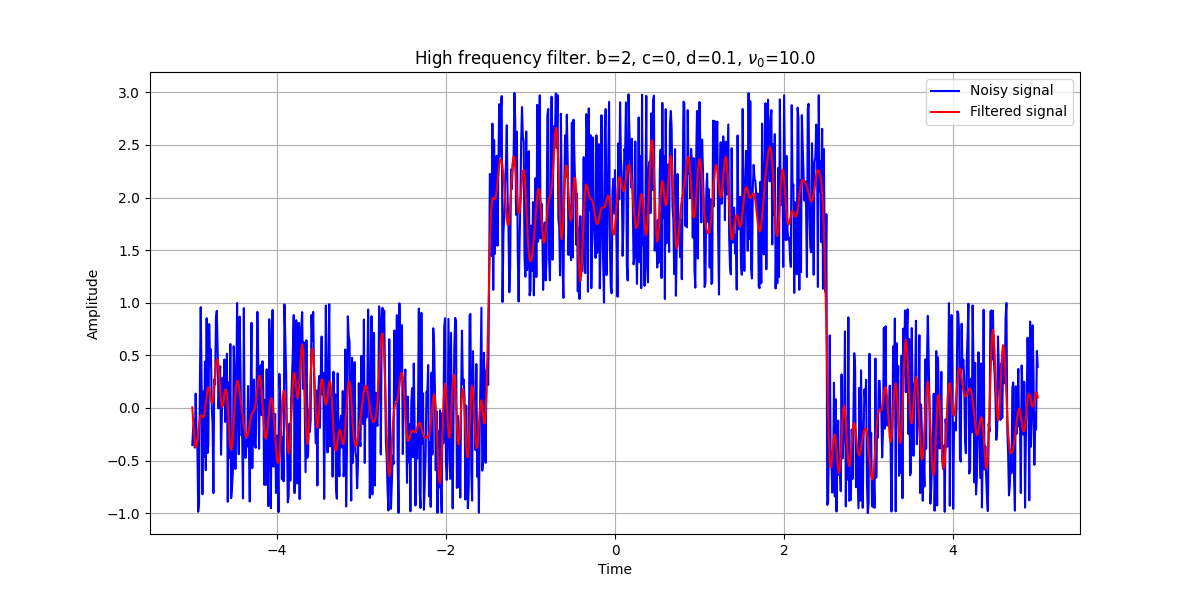
\includegraphics[scale=0.485]{3_u_flt_u_nohigh.png}
        \captionsetup{skip=0pt}
        \caption{График исходного и фильтрованного сигналов}
        \label{fig:fig5}
    \end{figure}
    \begin{figure}[!htb]
        \centering
        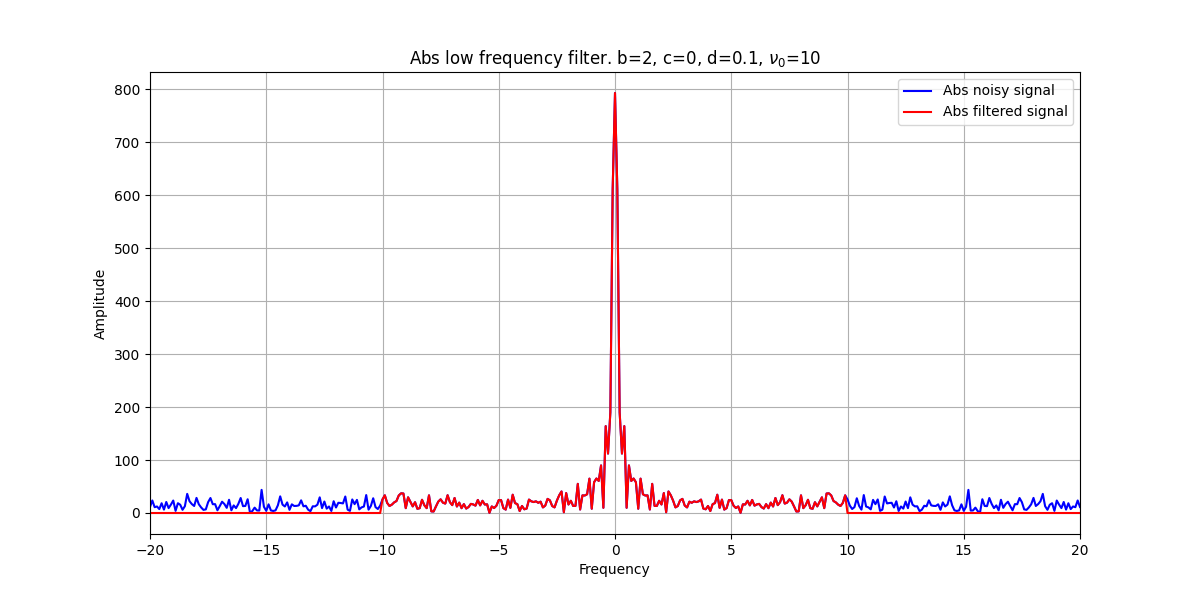
\includegraphics[scale=0.485]{3_abs_u_U_nohigh.png}
        \captionsetup{skip=0pt}
        \caption{График модуля Фурье-образа исходного и фильтрованного сигналов}
        \label{fig:fig6}
    \end{figure}
    \begin{figure}[!htb]
        \centering
        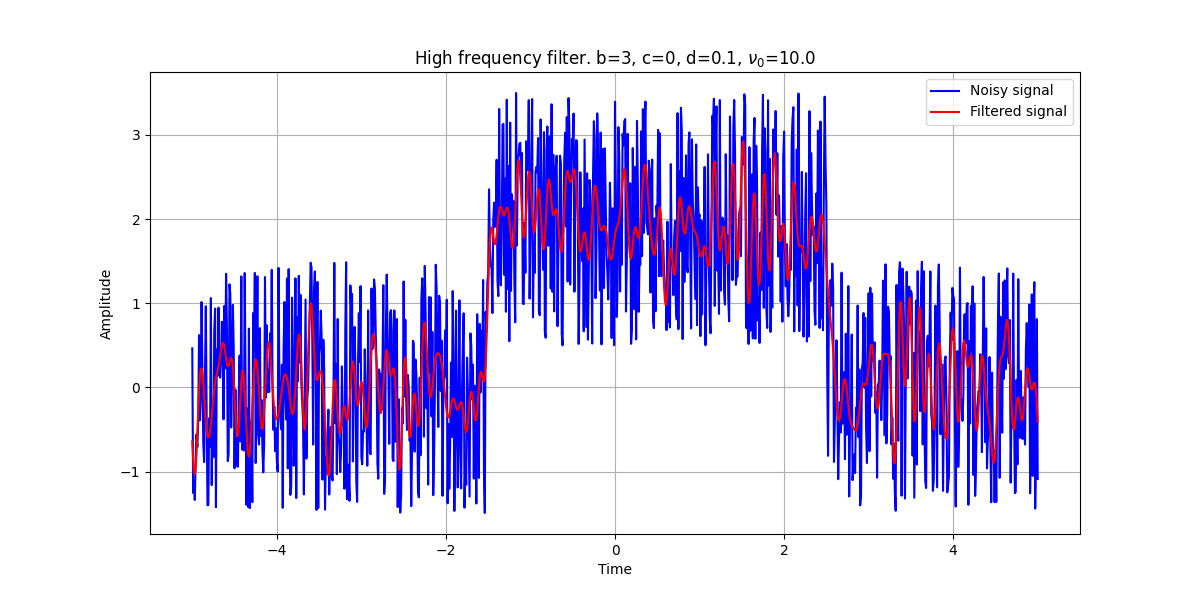
\includegraphics[scale=0.485]{5_u_flt_u_nohigh.png}
        \captionsetup{skip=0pt}
        \caption{График исходного и фильтрованного сигналов}
        \label{fig:fig7}
    \end{figure}
    \begin{figure}[!htb]
        \centering
        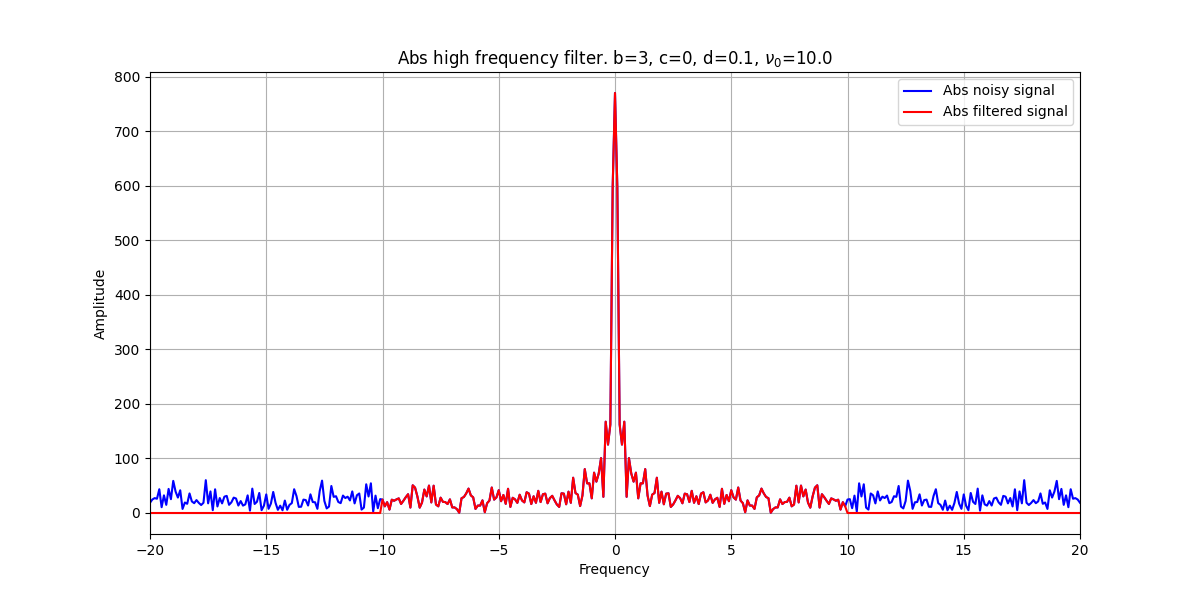
\includegraphics[scale=0.485]{5_abs_u_U_nohigh.png}
        \captionsetup{skip=0pt}
        \caption{График модуля Фурье-образа исходного и фильтрованного сигналов}
        \label{fig:fig8}
    \end{figure}
    \begin{figure}[!htb]
        \centering
        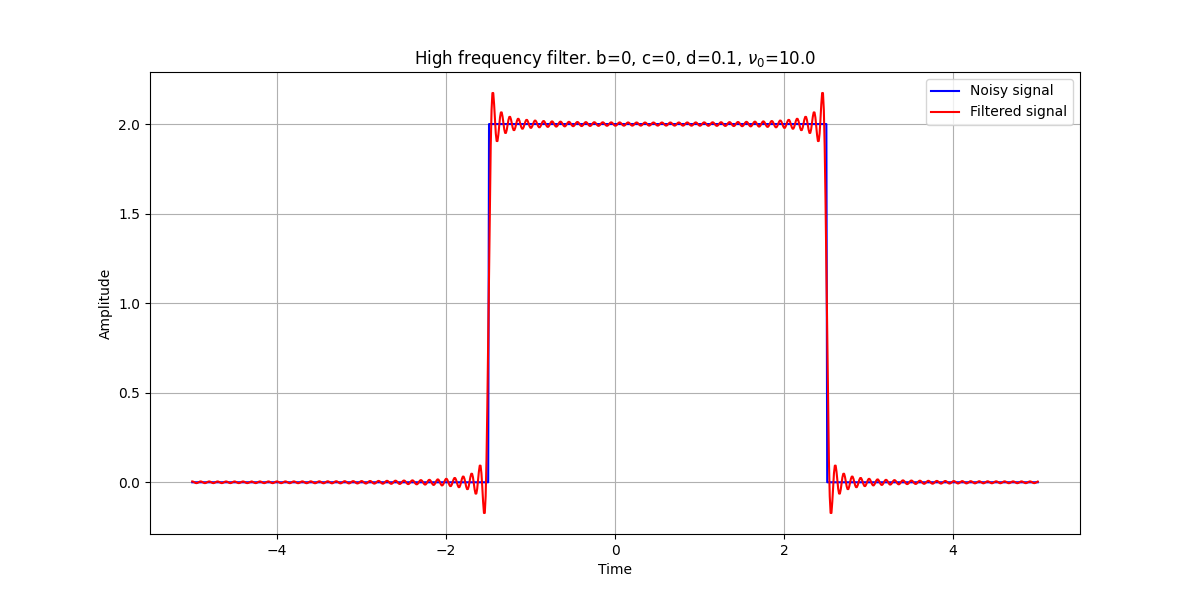
\includegraphics[scale=0.485]{4_u_flt_u_nohigh.png}
        \captionsetup{skip=0pt}
        \caption{График исходного и фильтрованного сигналов}
        \label{fig:fig9}
    \end{figure}
    \begin{figure}[!htb]
        \centering
        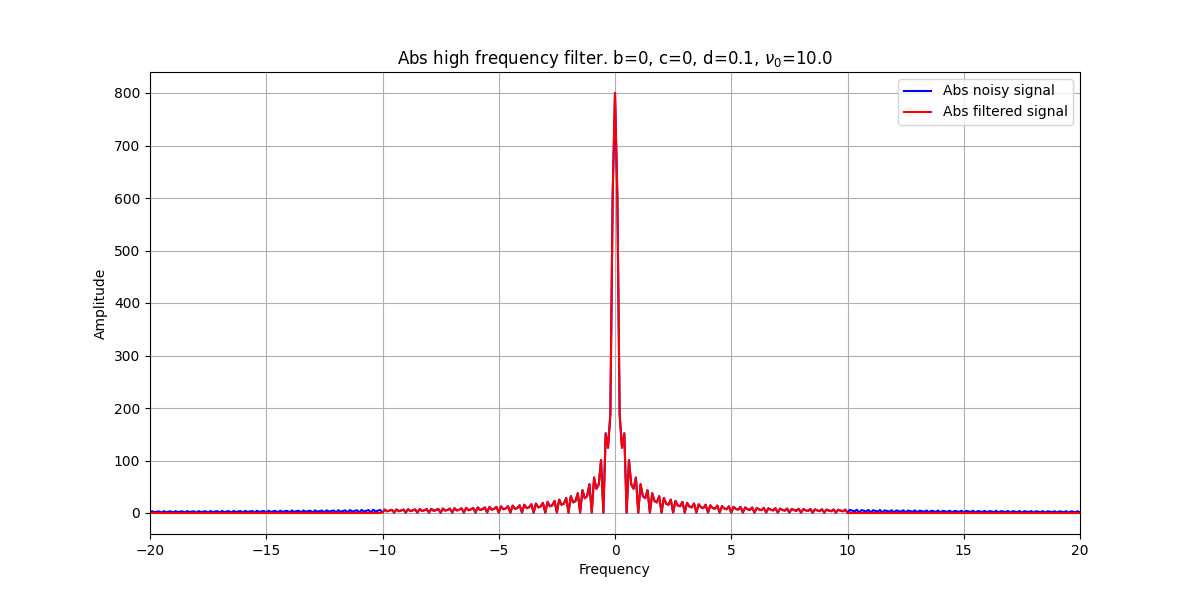
\includegraphics[scale=0.485]{4_abs_u_U_nohigh.png}
        \captionsetup{skip=0pt}
        \caption{График модуля Фурье-образа исходного и фильтрованного сигналов}
        \label{fig:fig10}
    \end{figure}
    \begin{figure}[!htb]
        \centering
        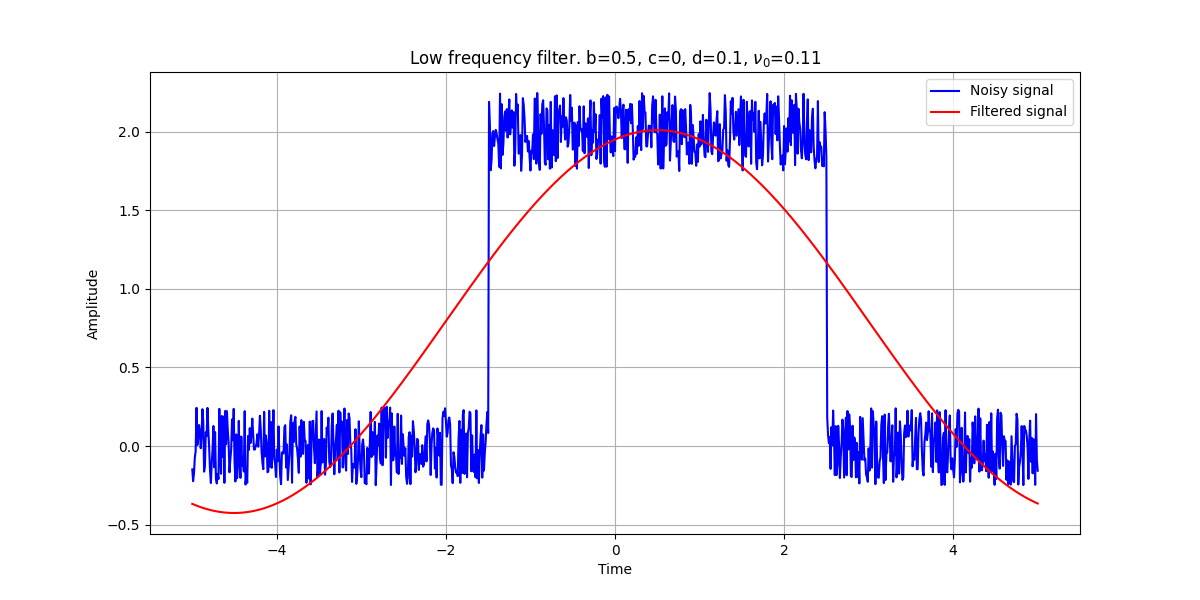
\includegraphics[scale=0.485]{11_u_flt_u_nohigh.png}
        \captionsetup{skip=0pt}
        \caption{График исходного и фильтрованного сигналов}
        \label{fig:fig11}
    \end{figure}
    \begin{figure}[!htb]
        \centering
        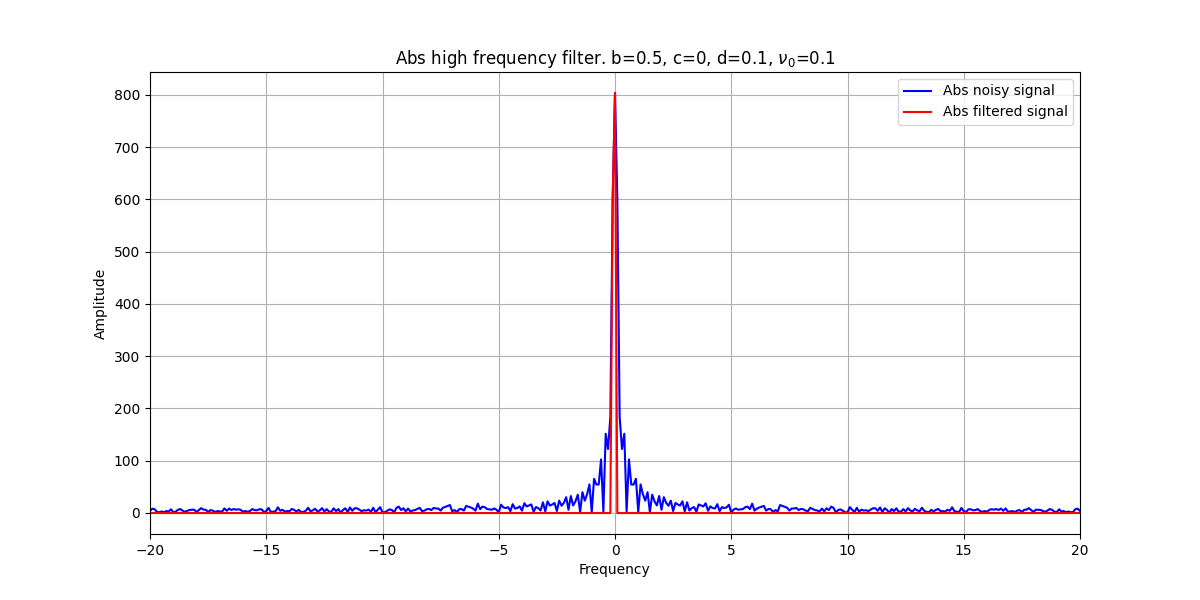
\includegraphics[scale=0.485]{11_abs_u_U_nohigh.png}
        \captionsetup{skip=0pt}
        \caption{График модуля Фурье-образа исходного и фильтрованного сигналов}
        \label{fig:fig12}
    \end{figure}
    \begin{figure}[!htb]
        \centering
        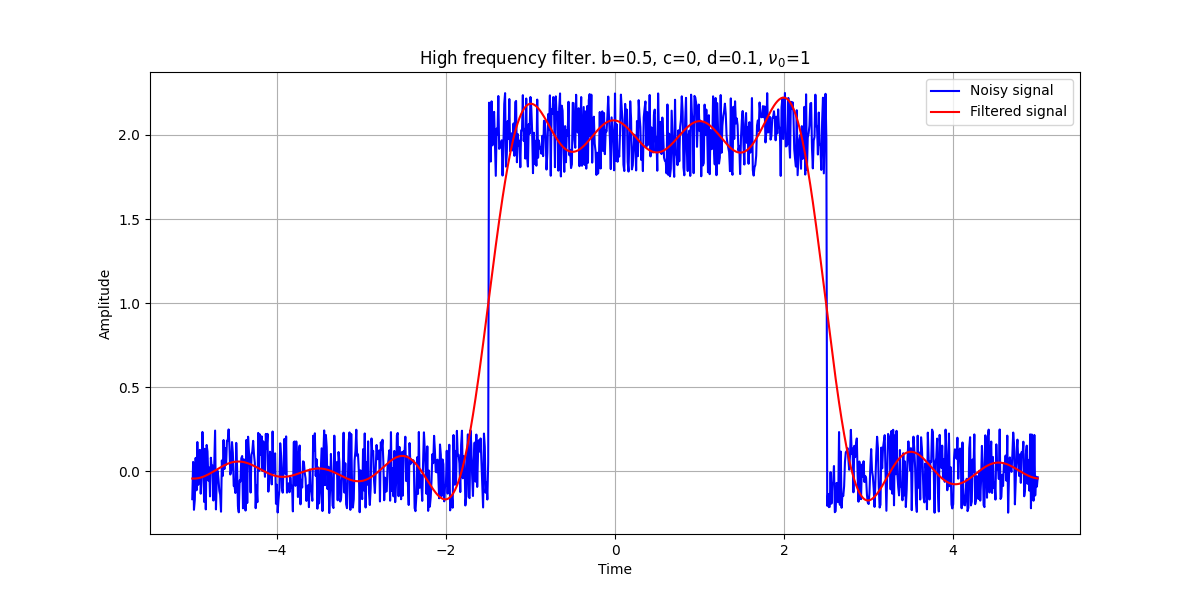
\includegraphics[scale=0.485]{12_u_flt_u_nohigh.png}
        \captionsetup{skip=0pt}
        \caption{График исходного и фильтрованного сигналов}
        \label{fig:fig13}
    \end{figure}
    \begin{figure}[!htb]
        \centering
        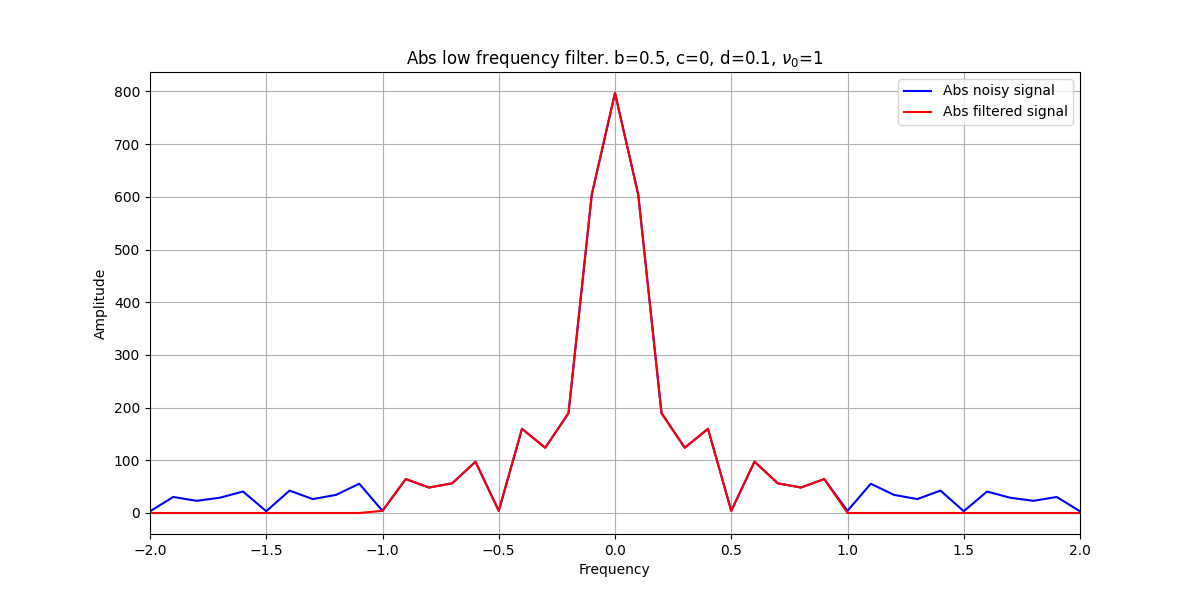
\includegraphics[scale=0.485]{12_abs_u_U_nohigh.png}
        \captionsetup{skip=0pt}
        \caption{График модуля Фурье-образа исходного и фильтрованного сигналов}
        \label{fig:fig14}
    \end{figure}
    \begin{figure}[!htb]
        \centering
        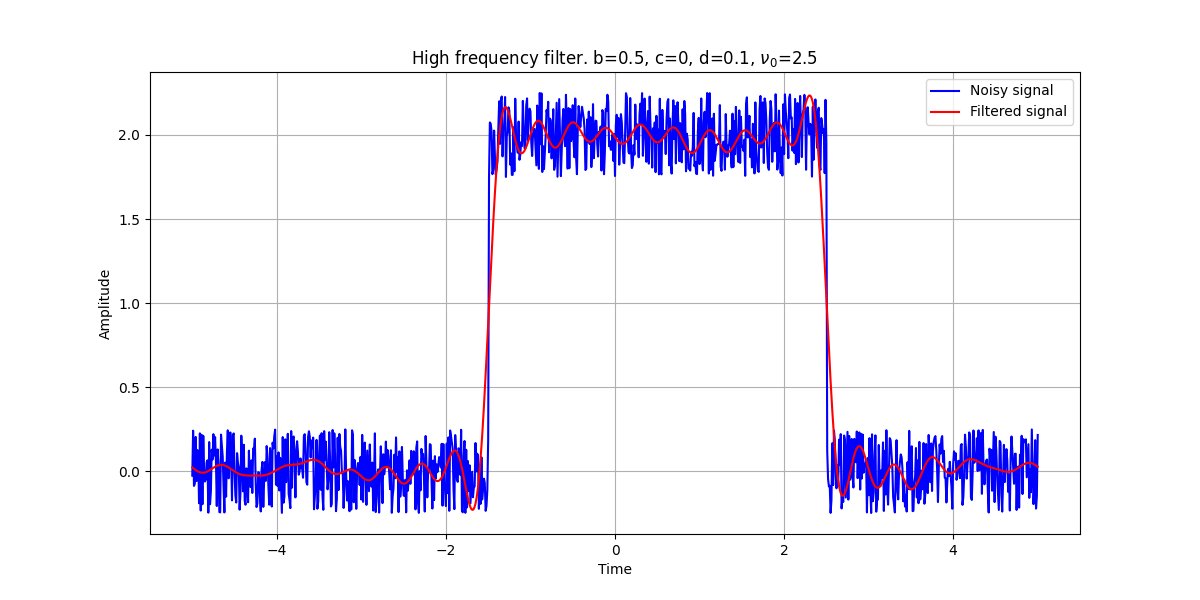
\includegraphics[scale=0.485]{13_u_flt_u_nohigh.png}
        \captionsetup{skip=0pt}
        \caption{График исходного и фильтрованного сигналов}
        \label{fig:fig15}
    \end{figure}
    \begin{figure}[!htb]
        \centering
        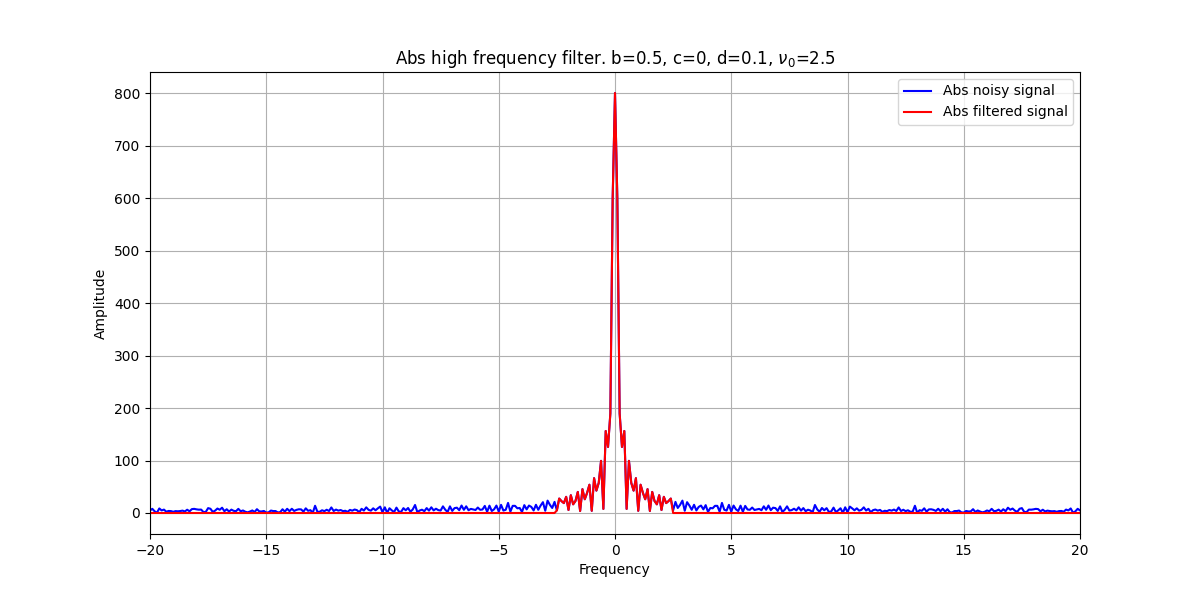
\includegraphics[scale=0.485]{13_abs_u_U_nohigh.png}
        \captionsetup{skip=0pt}
        \caption{График модуля Фурье-образа исходного и фильтрованного сигналов}
        \label{fig:fig16}
    \end{figure}
    \begin{figure}[!htb]
        \centering
        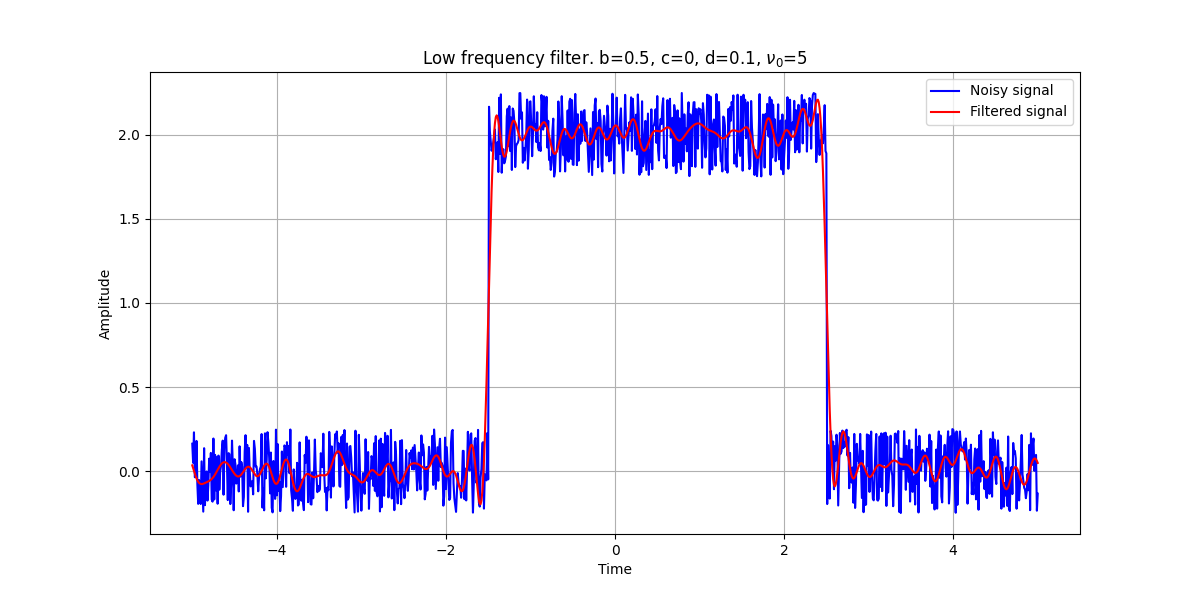
\includegraphics[scale=0.485]{8_u_flt_u_nohigh.png}
        \captionsetup{skip=0pt}
        \caption{График исходного и фильтрованного сигналов}
        \label{fig:fig17}
    \end{figure}
    \begin{figure}[!htb]
        \centering
        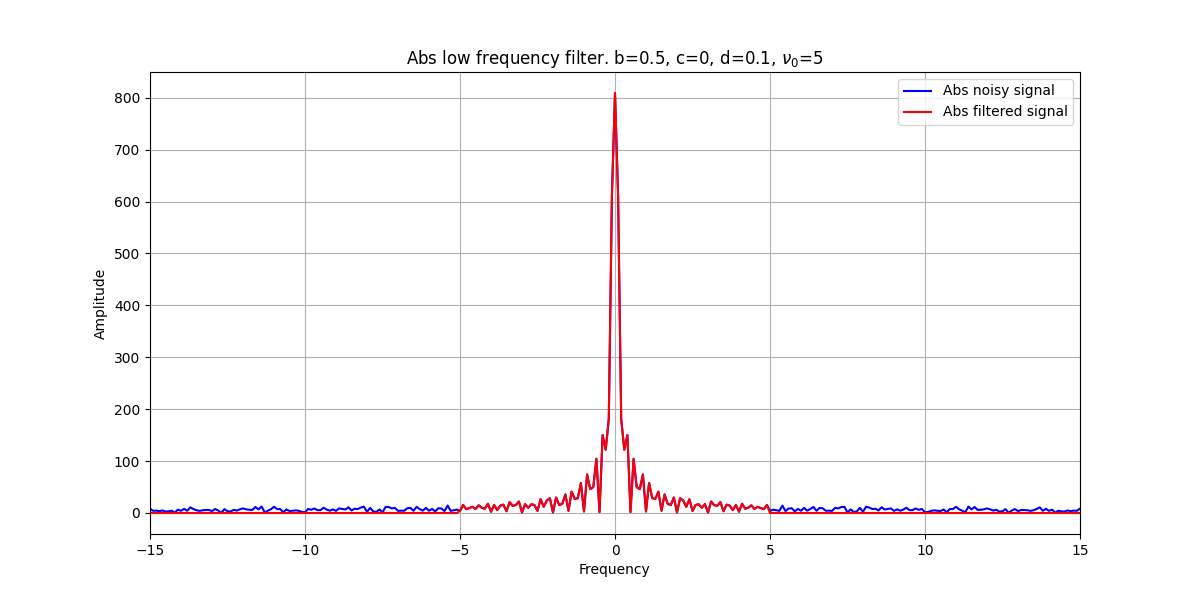
\includegraphics[scale=0.485]{8_abs_u_U_nohigh.png}
        \captionsetup{skip=0pt}
        \caption{График модуля Фурье-образа исходного и фильтрованного сигналов}
        \label{fig:fig18}
    \end{figure}
    \begin{figure}[!htb]
        \centering
        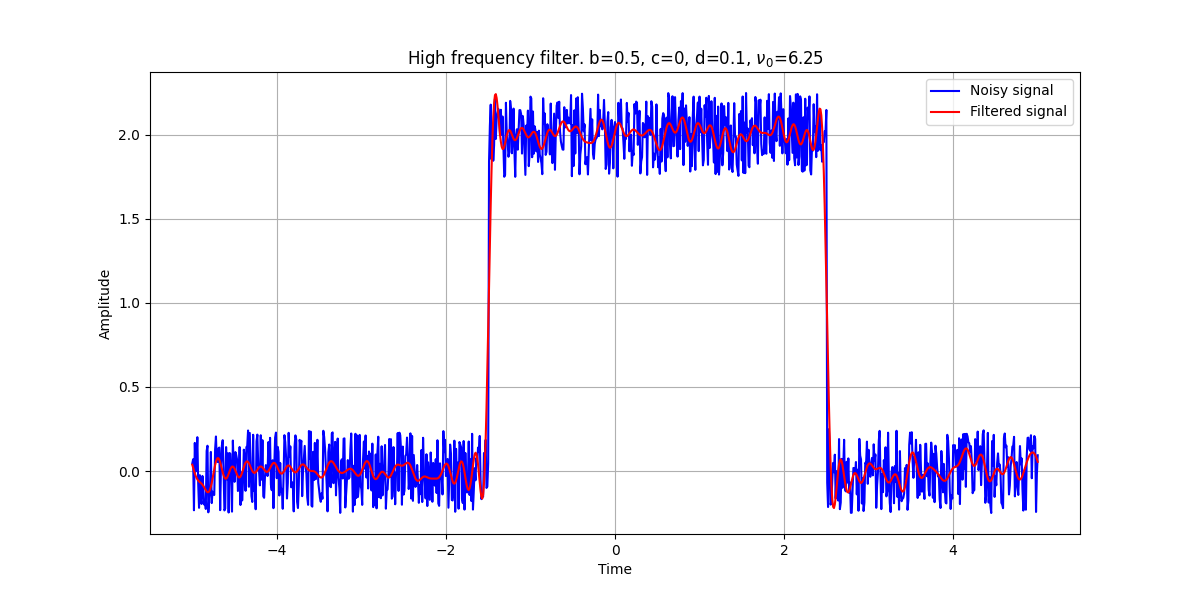
\includegraphics[scale=0.485]{7_u_flt_u_nohigh.png}
        \captionsetup{skip=0pt}
        \caption{График исходного и фильтрованного сигналов}
        \label{fig:fig19}
    \end{figure}
    \begin{figure}[!htb]
        \centering
        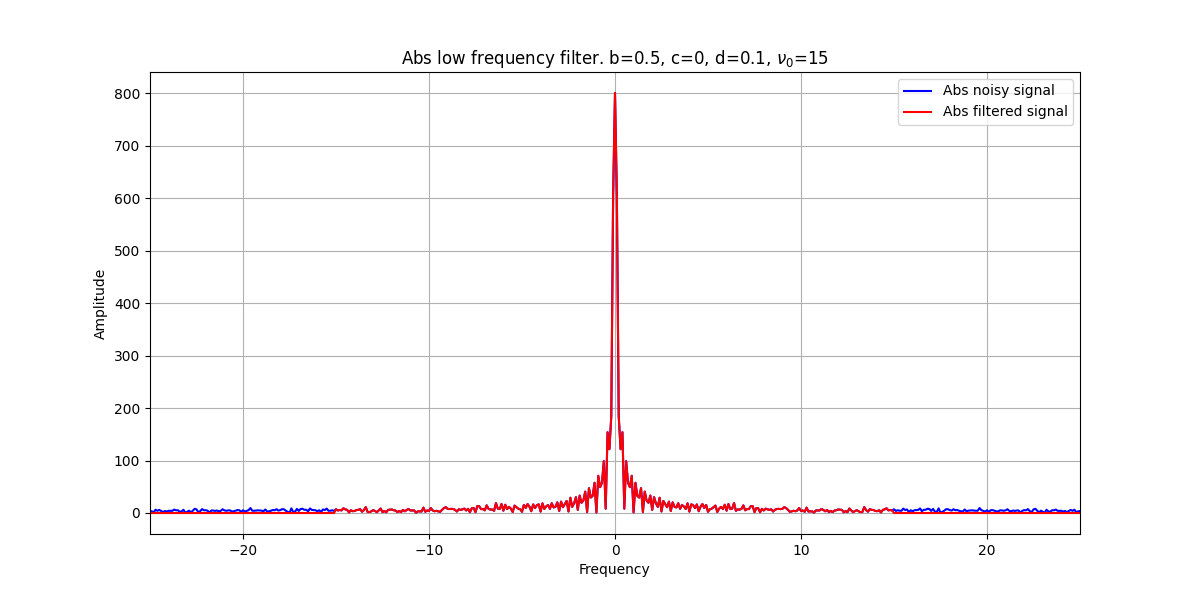
\includegraphics[scale=0.485]{7_abs_u_U_nohigh.png}
        \captionsetup{skip=0pt}
        \caption{График модуля Фурье-образа исходного и фильтрованного сигналов}
        \label{fig:fig20}
    \end{figure}
    \begin{figure}[!htb]
        \centering
        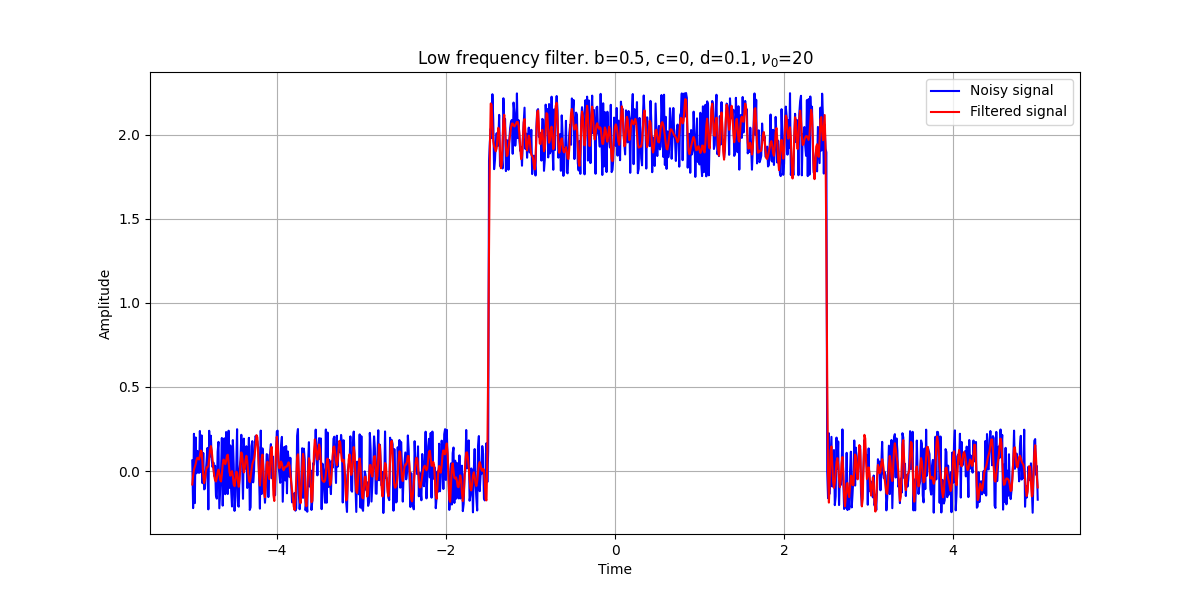
\includegraphics[scale=0.485]{6_u_flt_u_nohigh.png}
        \captionsetup{skip=0pt}
        \caption{График исходного и фильтрованного сигналов}
        \label{fig:fig21}
    \end{figure}
    \begin{figure}[!htb]
        \centering
        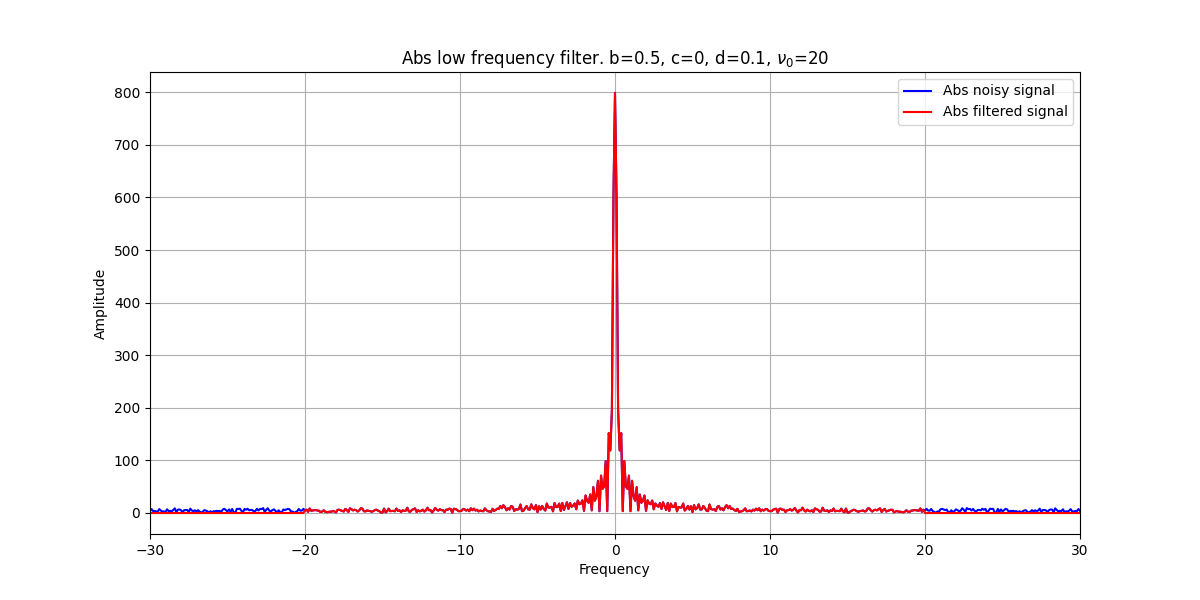
\includegraphics[scale=0.485]{6_abs_u_U_nohigh.png}
        \captionsetup{skip=0pt}
        \caption{График модуля Фурье-образа исходного и фильтрованного сигналов}
        \label{fig:fig22}
    \end{figure}
    \begin{figure}[!htb]
        \centering
        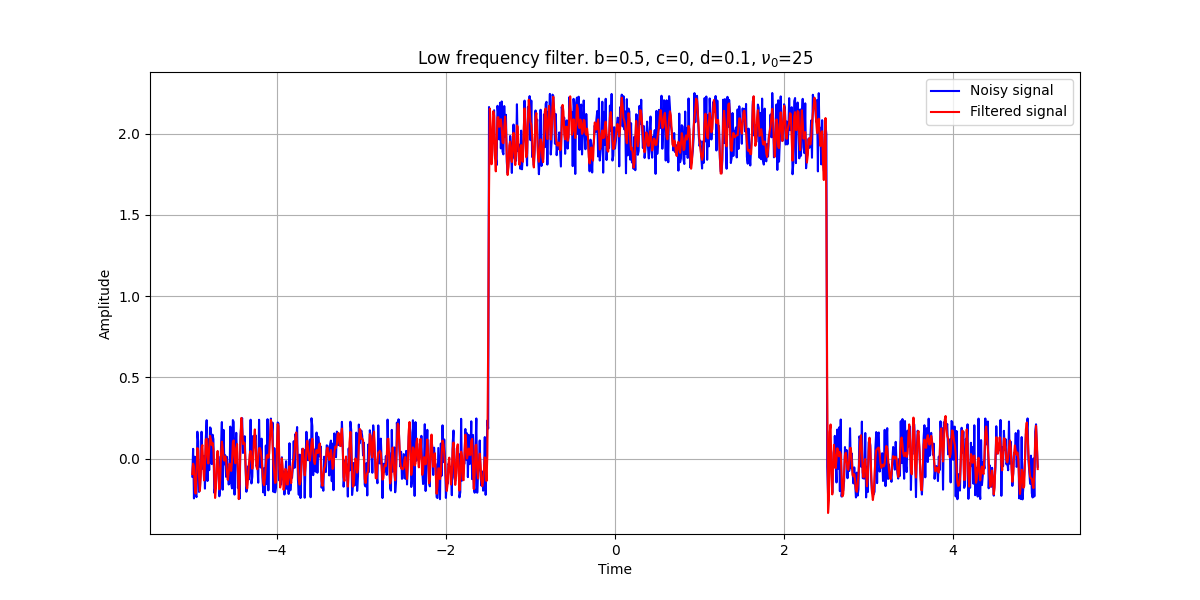
\includegraphics[scale=0.485]{10_u_flt_u_nohigh.png}
        \captionsetup{skip=0pt}
        \caption{График исходного и фильтрованного сигналов}
        \label{fig:fig23}
    \end{figure}
    \begin{figure}[!htb]
        \centering
        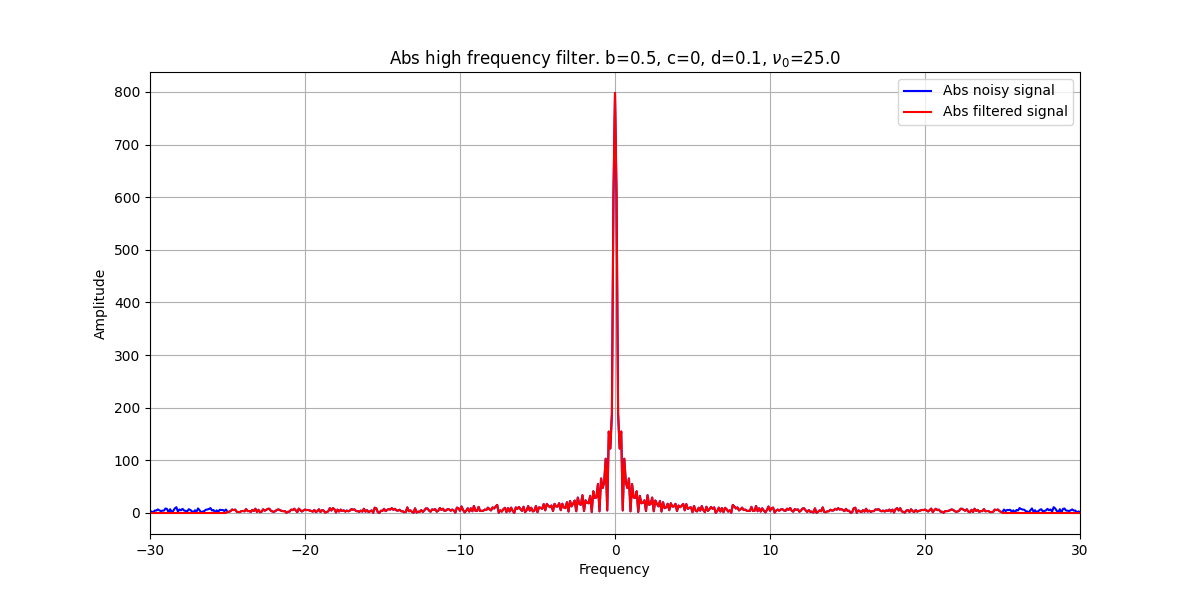
\includegraphics[scale=0.485]{10_abs_u_U_nohigh.png}
        \captionsetup{skip=0pt}
        \caption{График модуля Фурье-образа исходного и фильтрованного сигналов}
        \label{fig:fig24}
    \end{figure}
    \begin{figure}[!htb]
        \centering
        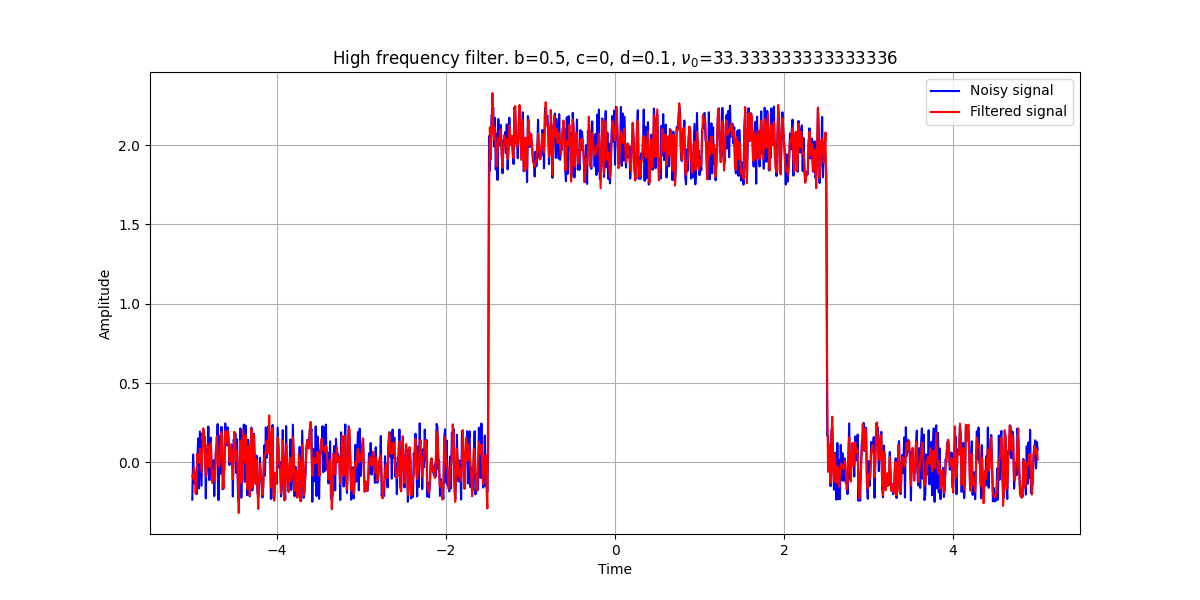
\includegraphics[scale=0.485]{9_u_flt_u_nohigh.png}
        \captionsetup{skip=0pt}
        \caption{График исходного и фильтрованного сигналов}
        \label{fig:fig25}
    \end{figure}
    \begin{figure}[!htb]
        \centering
        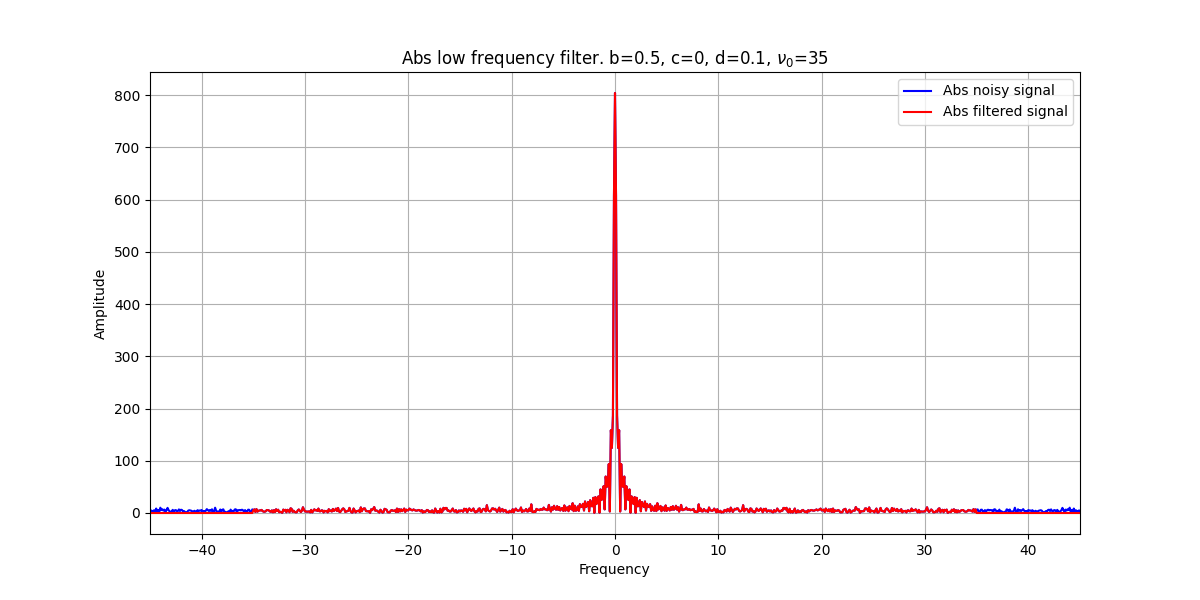
\includegraphics[scale=0.485]{9_abs_u_U_nohigh.png}
        \captionsetup{skip=0pt}
        \caption{График модуля Фурье-образа исходного и фильтрованного сигналов}
        \label{fig:fig26}
    \end{figure}


    Исходя из графиков можно сделать вывод, что значение параметра $b$ отвечает за амплитуду каждой волны.
    Чем больше значение $b$, тем зашумленнее, <<грязнее>> выглядит сигнал, так как амплитуды волн возрастают.
    Фильтрованный сигнал при больших значениях $b$ также имеет более глубокие ямы и высокие подъемы, то есть
    испытывает увеличение амплитуды. Наглядно такое возрастание можно наблюдать на графиках модуля Фурье-образа
    исходного и фильтрованного сигналов -- на рисунке \ref{fig:fig2} амплитуды больше прижимаются к линии 
    $A=0$, а на рисунке \ref{fig:fig8} они больше стремятся к линии $A=50$, где $A$ -- амплитуда. Само значение
    параметра $b$ не влияет на эффективность фильтрации в локальном смысле, то есть из плохого зашумленного сигнала
    получается фильтрованный плохой сигнал, но в глобальном смысле чем меньше значение $b$, тем чище сигнал и тем лучше
    сама фильтрация. При $b=0$ получается особый случай -- сигнал превращается в прямоугольную функцию, а фильтрованный
    сигнал выглядит как ее аппроксимация.


    Больше всего влияния на эффективность фильтрации оказывает частота среза $\nu_0$. Этот параметр необходимо подобрать
    так, чтобы оставались только те частоты, которые имеют заметно более высокую амплитуду по сравнению с остальными.
    Чем меньше частота среза $\nu_0$, тем заметно лучше фильтрация, однако, если взять слишком маленькое значение $\nu_0$,
    то фильтрация будет слишком сильной и мы потеряем большую часть значащих частот в сигнале, что можно увидеть на рисунке
    \ref{fig:fig11}. Если взять слишком больше значение $\nu_0$, то фильтрация будет не очень эффективной (см. рис. \ref{fig:fig25}).


    \subsection{Убираем низкие частоты.}
    Рассмотрим графики, где в некоторой окресности точки $\nu=0$ обнулим все значения частот Фурье-образа, таким образом избавившись
    от наивысших амплитуд. Окресность будет настраиваться выбором диапазона частот $[-\nu_0,\nu_0]$, где фильтр будет обнулять все частоты, 
    что входят в него. Также рассмотрим поведение фильтрации при различных параметрах $b,\,c,\,d$.


    Далее будут приведены рисунки полученных графиков. На каждом графике подписаны выбранные значения $b,\,c,\,d,\,\nu_0$. 
    Также отмечена легенда -- синим цветом обозначается оригинальный сигнал, красным фильтрованный.


    % todo анализ
    \begin{figure}[!htb]
        \centering
        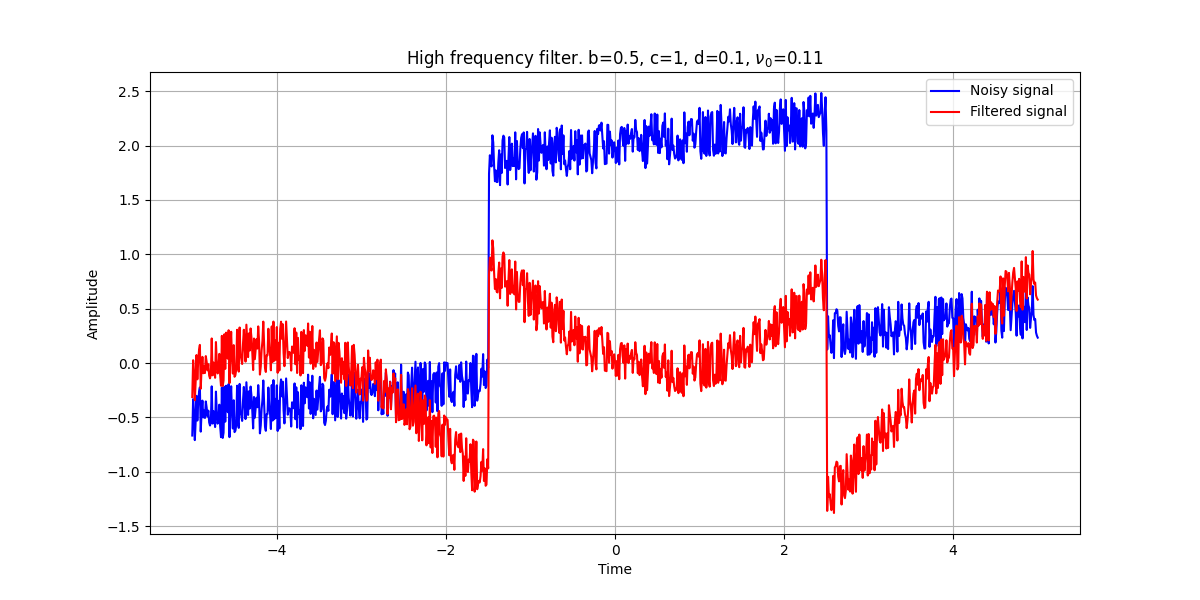
\includegraphics[scale=0.485]{1_u_flt_u_nolow.png}
        \captionsetup{skip=0pt}
        \caption{График исходного и фильтрованного сигналов}
        \label{fig:fig27}
    \end{figure}
    \begin{figure}[!htb]
        \centering
        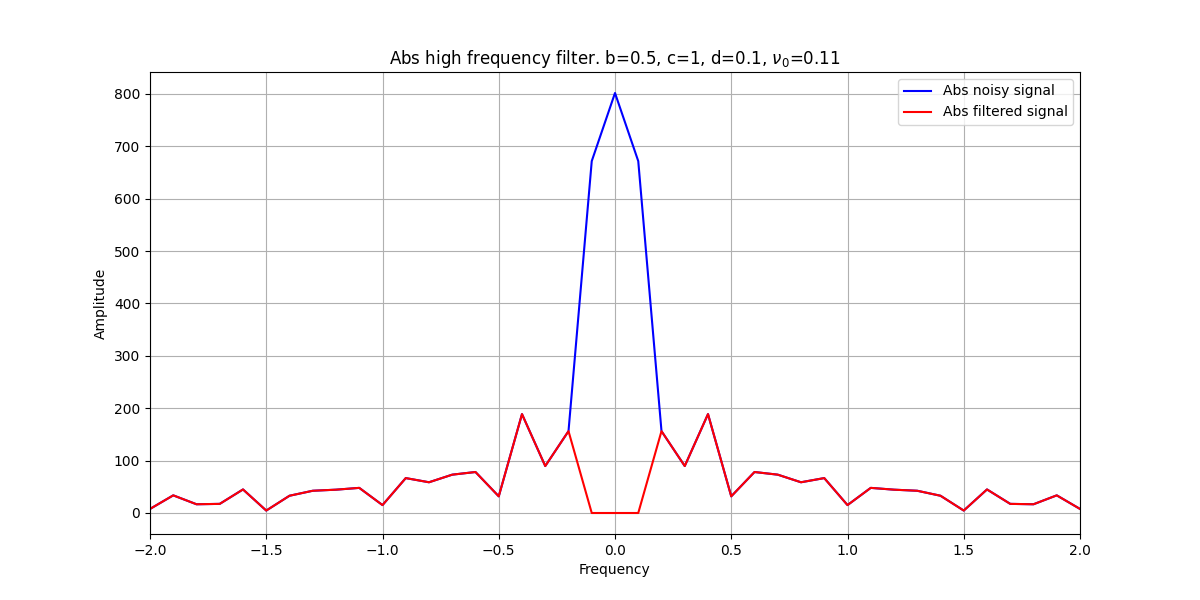
\includegraphics[scale=0.485]{1_abs_u_U_nolow.png}
        \captionsetup{skip=0pt}
        \caption{График модуля Фурье-образа исходного и фильтрованного сигналов}
        \label{fig:fig28}
    \end{figure}
    \begin{figure}[!htb]
        \centering
        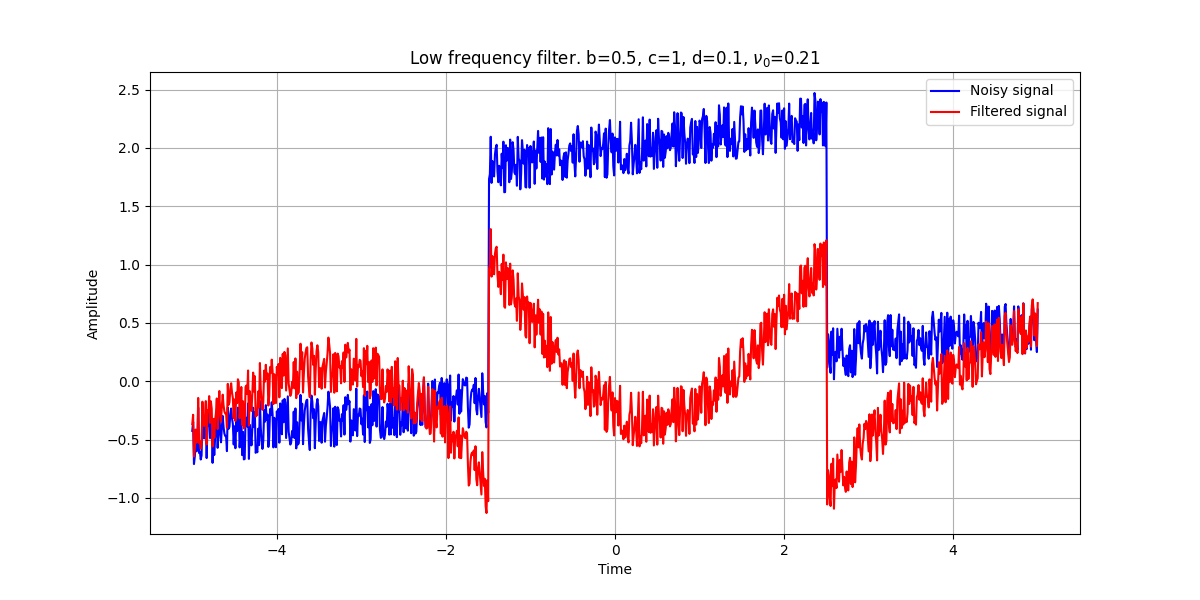
\includegraphics[scale=0.485]{2_u_flt_u_nolow.png}
        \captionsetup{skip=0pt}
        \caption{График исходного и фильтрованного сигналов}
        \label{fig:fig29}
    \end{figure}
    \begin{figure}[!htb]
        \centering
        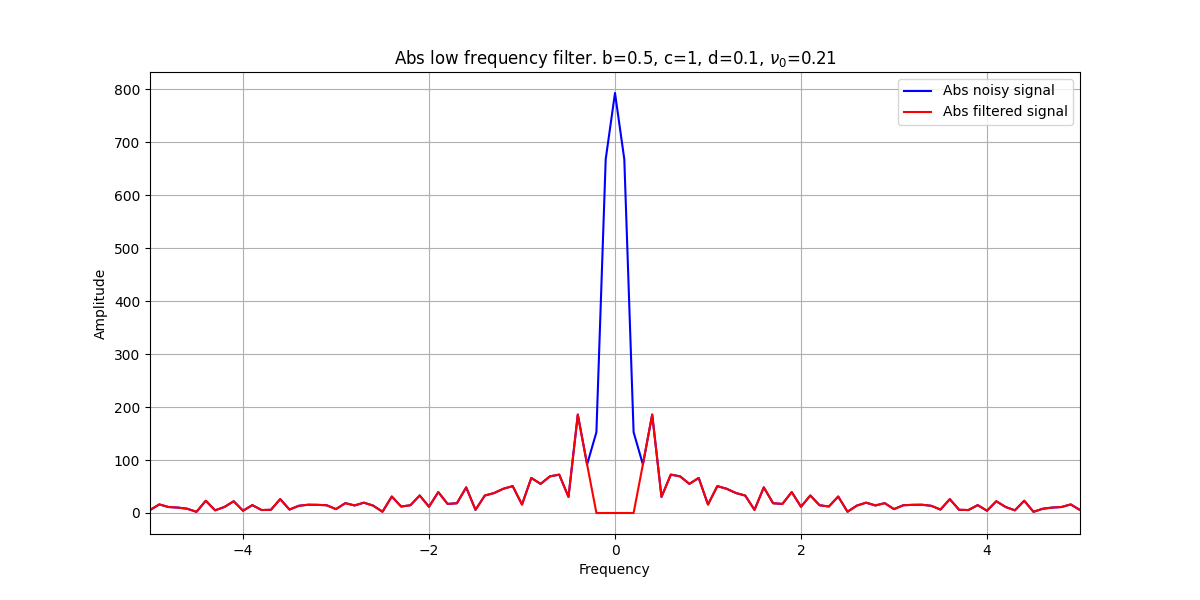
\includegraphics[scale=0.485]{2_abs_u_U_nolow.png}
        \captionsetup{skip=0pt}
        \caption{График модуля Фурье-образа исходного и фильтрованного сигналов}
        \label{fig:fig30}
    \end{figure}
    \begin{figure}[!htb]
        \centering
        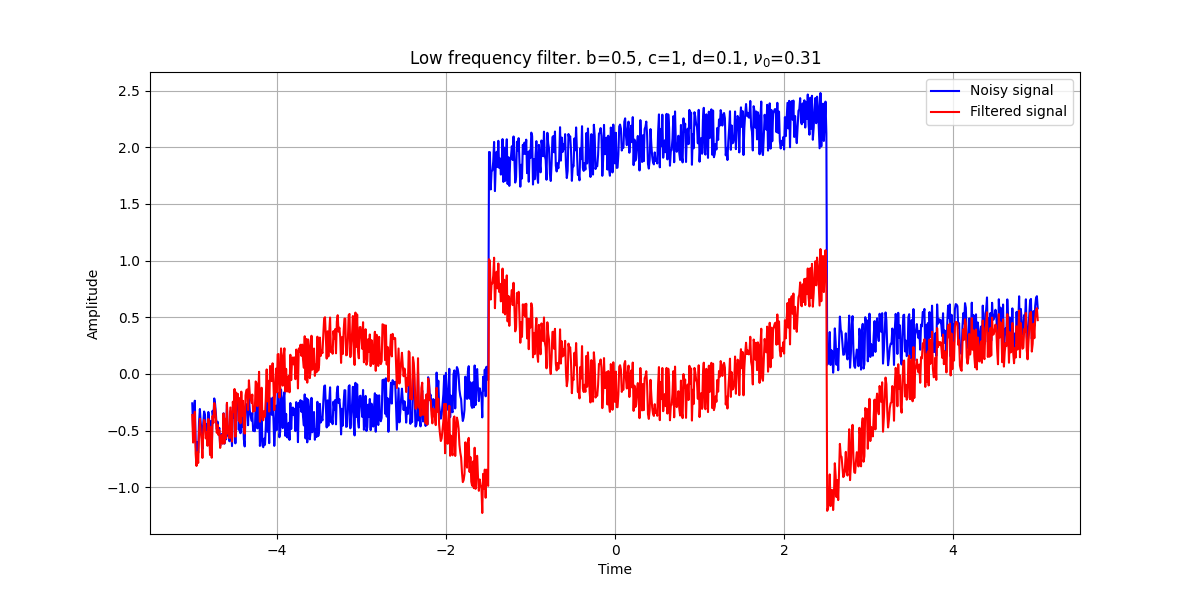
\includegraphics[scale=0.485]{3_u_flt_u_nolow.png}
        \captionsetup{skip=0pt}
        \caption{График исходного и фильтрованного сигналов}
        \label{fig:fig31}
    \end{figure}
    \begin{figure}[!htb]
        \centering
        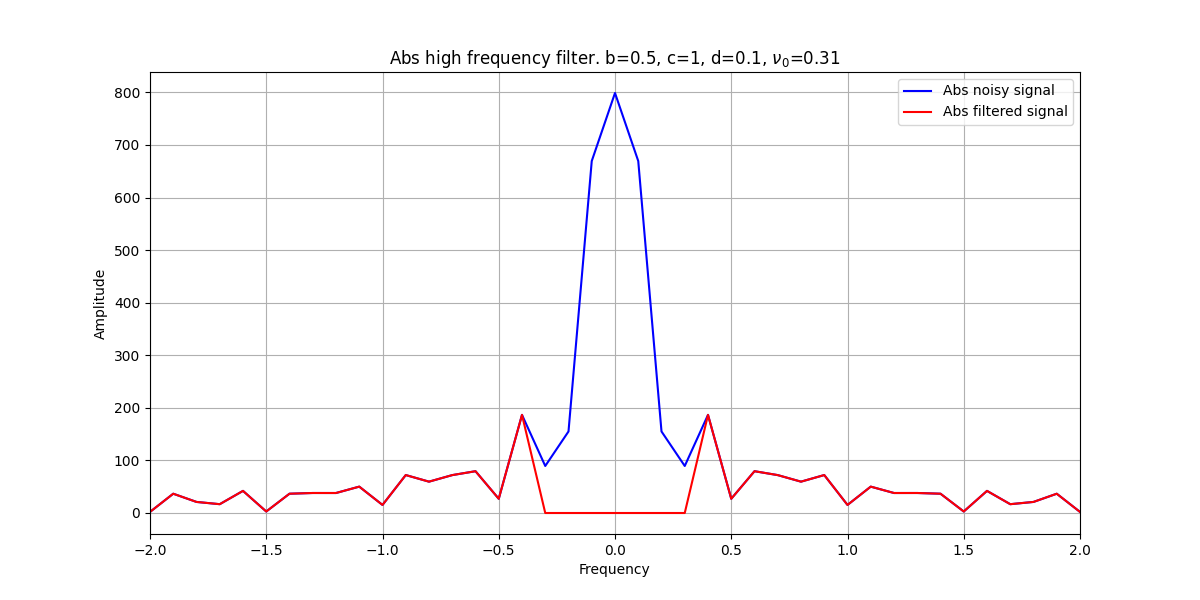
\includegraphics[scale=0.485]{3_abs_u_U_nolow.png}
        \captionsetup{skip=0pt}
        \caption{График модуля Фурье-образа исходного и фильтрованного сигналов}
        \label{fig:fig32}
    \end{figure}
    \begin{figure}[!htb]
        \centering
        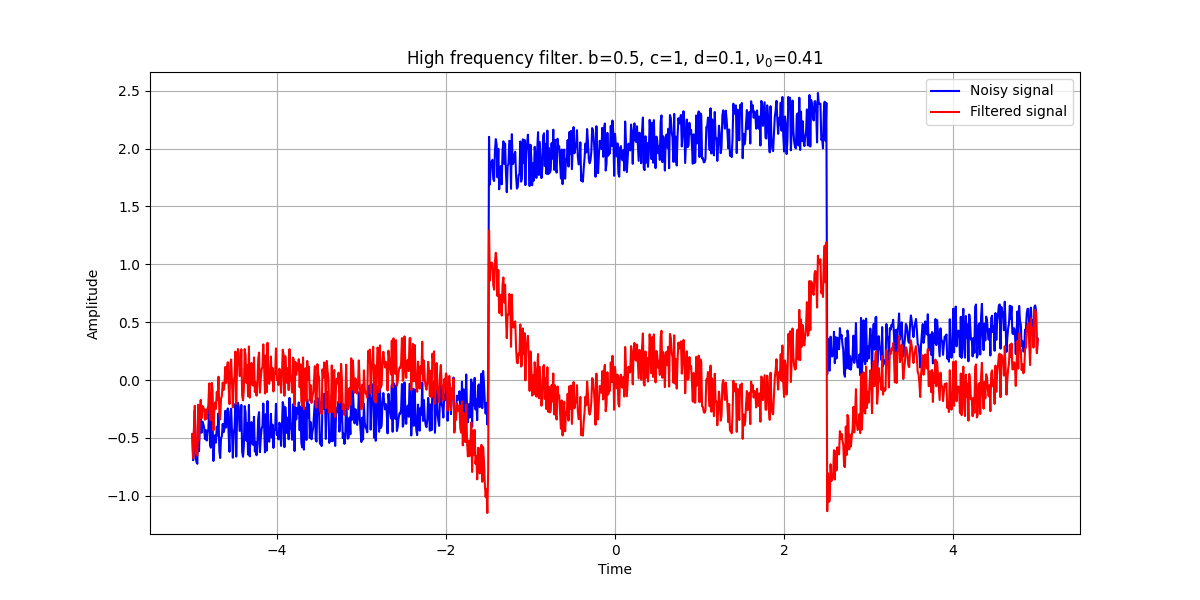
\includegraphics[scale=0.485]{4_u_flt_u_nolow.png}
        \captionsetup{skip=0pt}
        \caption{График исходного и фильтрованного сигналов}
        \label{fig:fig33}
    \end{figure}
    \begin{figure}[!htb]
        \centering
        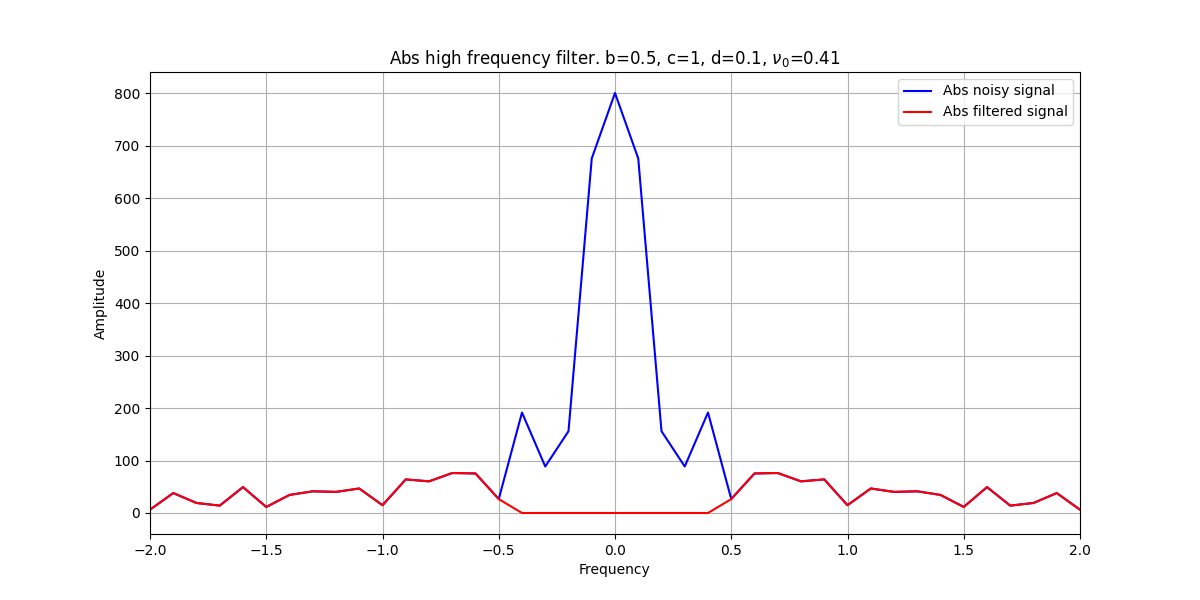
\includegraphics[scale=0.485]{4_abs_u_U_nolow.png}
        \captionsetup{skip=0pt}
        \caption{График модуля Фурье-образа исходного и фильтрованного сигналов}
        \label{fig:fig34}
    \end{figure}
    \begin{figure}[!htb]
        \centering
        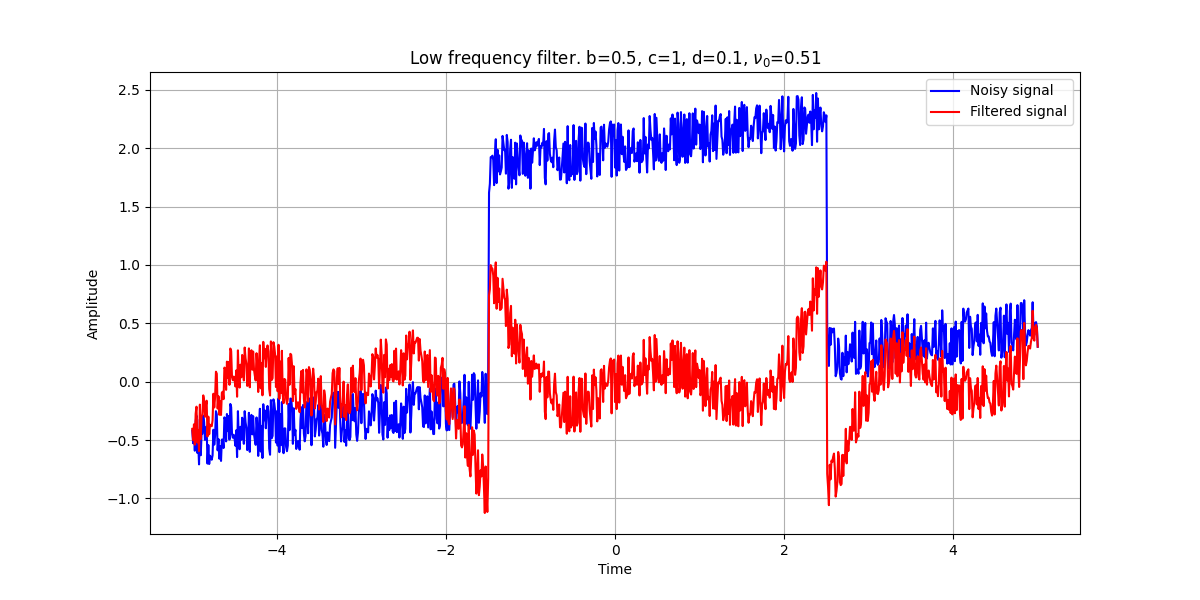
\includegraphics[scale=0.485]{5_u_flt_u_nolow.png}
        \captionsetup{skip=0pt}
        \caption{График исходного и фильтрованного сигналов}
        \label{fig:fig35}
    \end{figure}
    \begin{figure}[!htb]
        \centering
        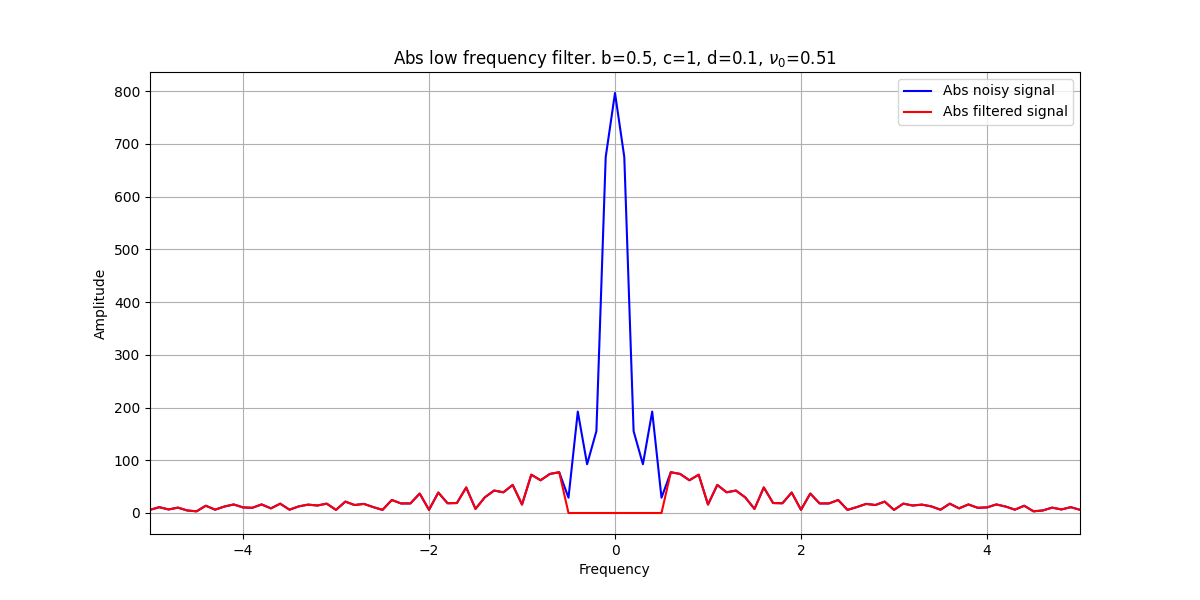
\includegraphics[scale=0.485]{5_abs_u_U_nolow.png}
        \captionsetup{skip=0pt}
        \caption{График модуля Фурье-образа исходного и фильтрованного сигналов}
        \label{fig:fig36}
    \end{figure}
    \begin{figure}[!htb]
        \centering
        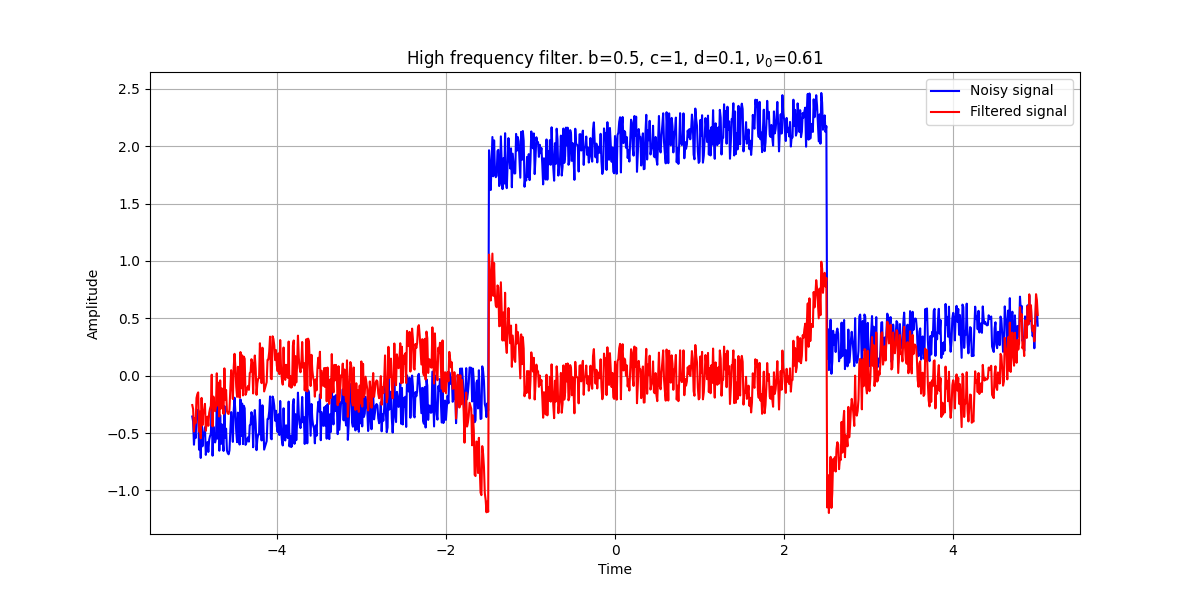
\includegraphics[scale=0.485]{6_u_flt_u_nolow.png}
        \captionsetup{skip=0pt}
        \caption{График исходного и фильтрованного сигналов}
        \label{fig:fig37}
    \end{figure}
    \begin{figure}[!htb]
        \centering
        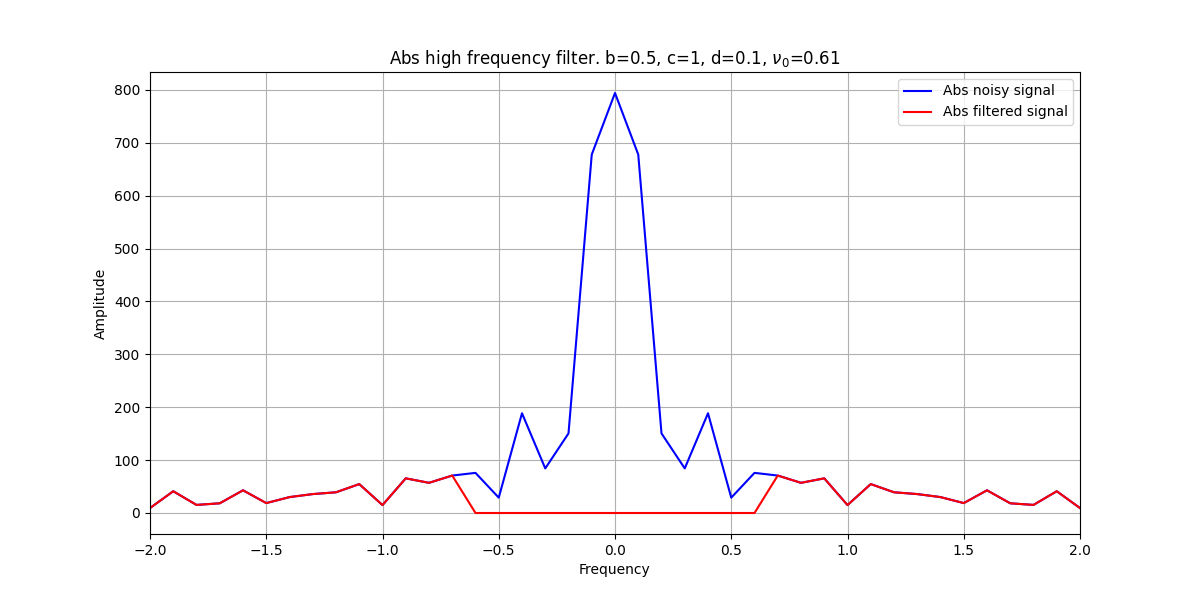
\includegraphics[scale=0.485]{6_abs_u_U_nolow.png}
        \captionsetup{skip=0pt}
        \caption{График модуля Фурье-образа исходного и фильтрованного сигналов}
        \label{fig:fig38}
    \end{figure}
    \begin{figure}[!htb]
        \centering
        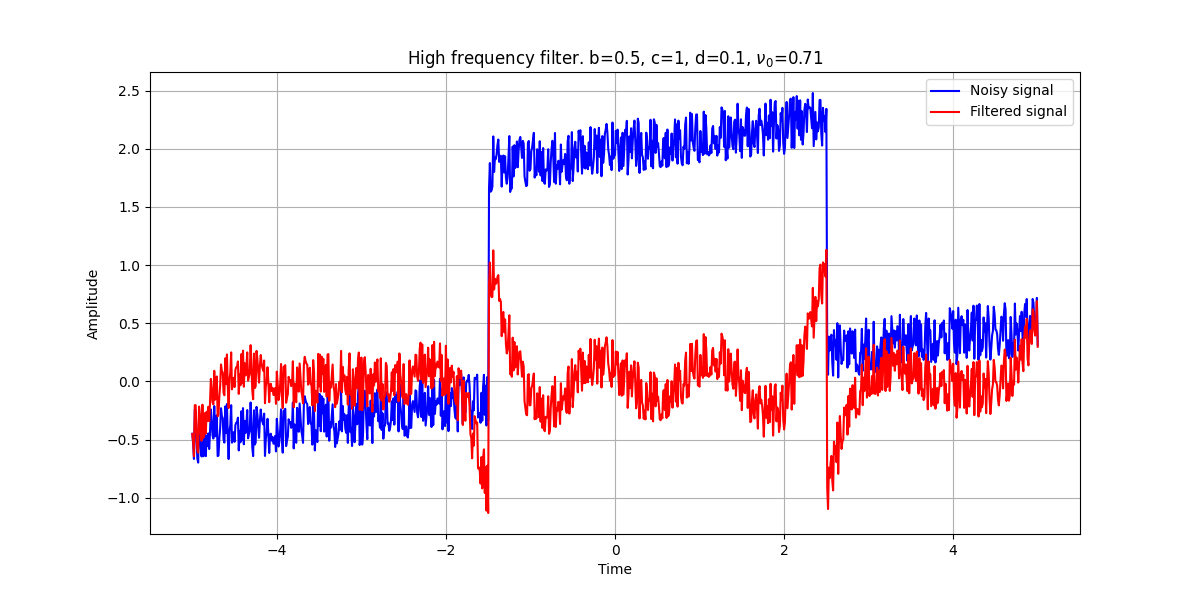
\includegraphics[scale=0.485]{7_u_flt_u_nolow.png}
        \captionsetup{skip=0pt}
        \caption{График исходного и фильтрованного сигналов}
        \label{fig:fig39}
    \end{figure}
    \begin{figure}[!htb]
        \centering
        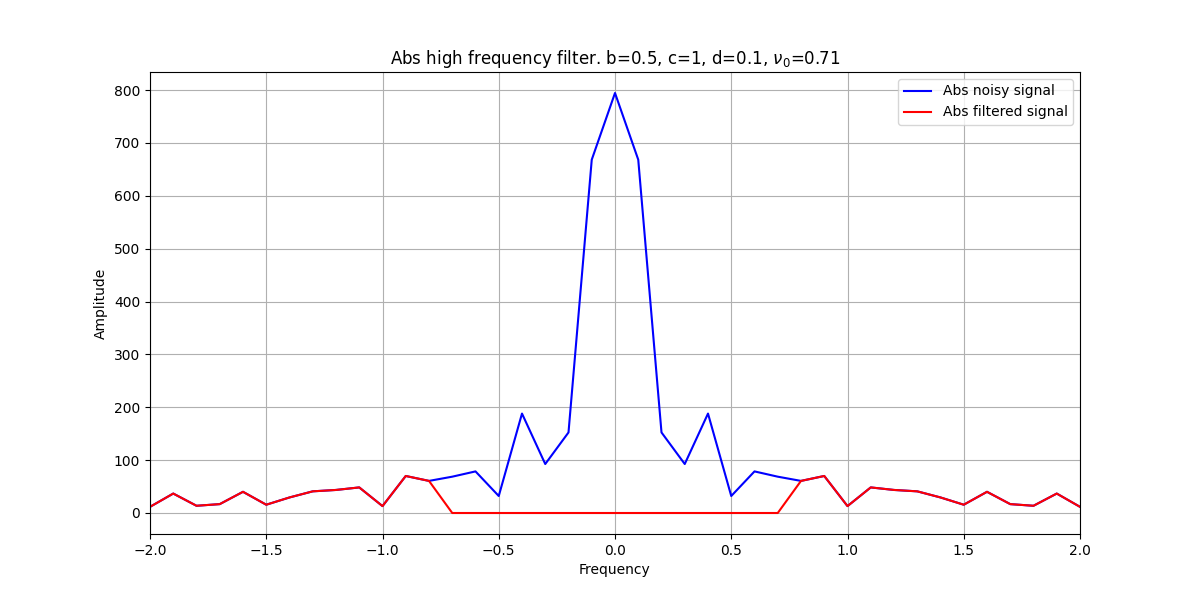
\includegraphics[scale=0.485]{7_abs_u_U_nolow.png}
        \captionsetup{skip=0pt}
        \caption{График модуля Фурье-образа исходного и фильтрованного сигналов}
        \label{fig:fig40}
    \end{figure}
    \begin{figure}[!htb]
        \centering
        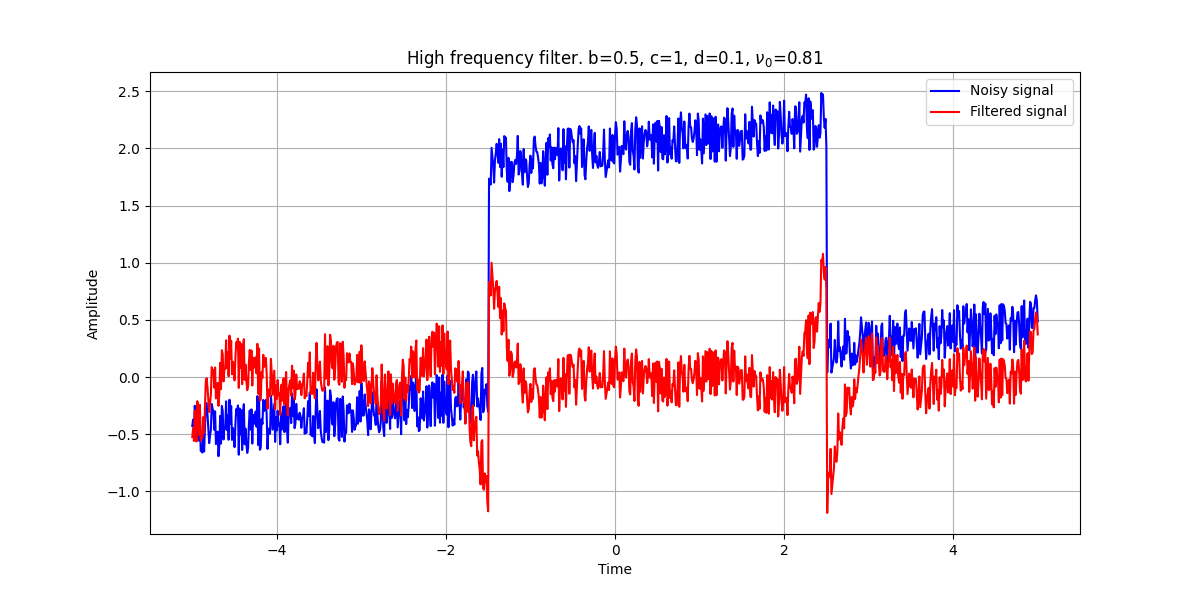
\includegraphics[scale=0.485]{8_u_flt_u_nolow.png}
        \captionsetup{skip=0pt}
        \caption{График исходного и фильтрованного сигналов}
        \label{fig:fig41}
    \end{figure}
    \begin{figure}[!htb]
        \centering
        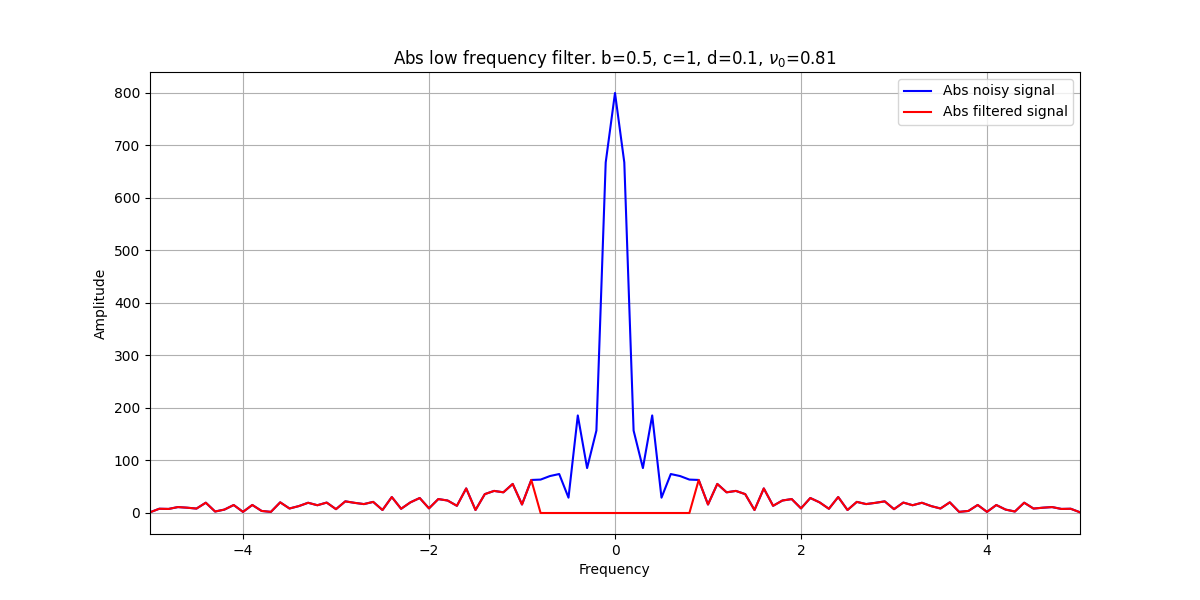
\includegraphics[scale=0.485]{8_abs_u_U_nolow.png}
        \captionsetup{skip=0pt}
        \caption{График модуля Фурье-образа исходного и фильтрованного сигналов}
        \label{fig:fig42}
    \end{figure}
    \begin{figure}[!htb]
        \centering
        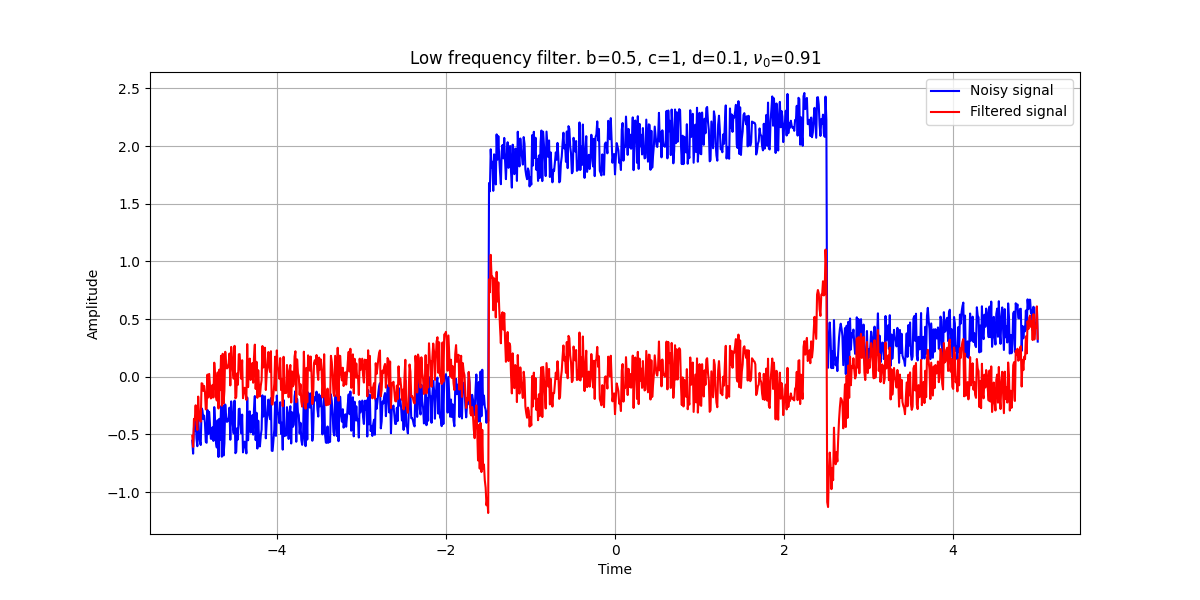
\includegraphics[scale=0.485]{9_u_flt_u_nolow.png}
        \captionsetup{skip=0pt}
        \caption{График исходного и фильтрованного сигналов}
        \label{fig:fig43}
    \end{figure}
    \begin{figure}[!htb]
        \centering
        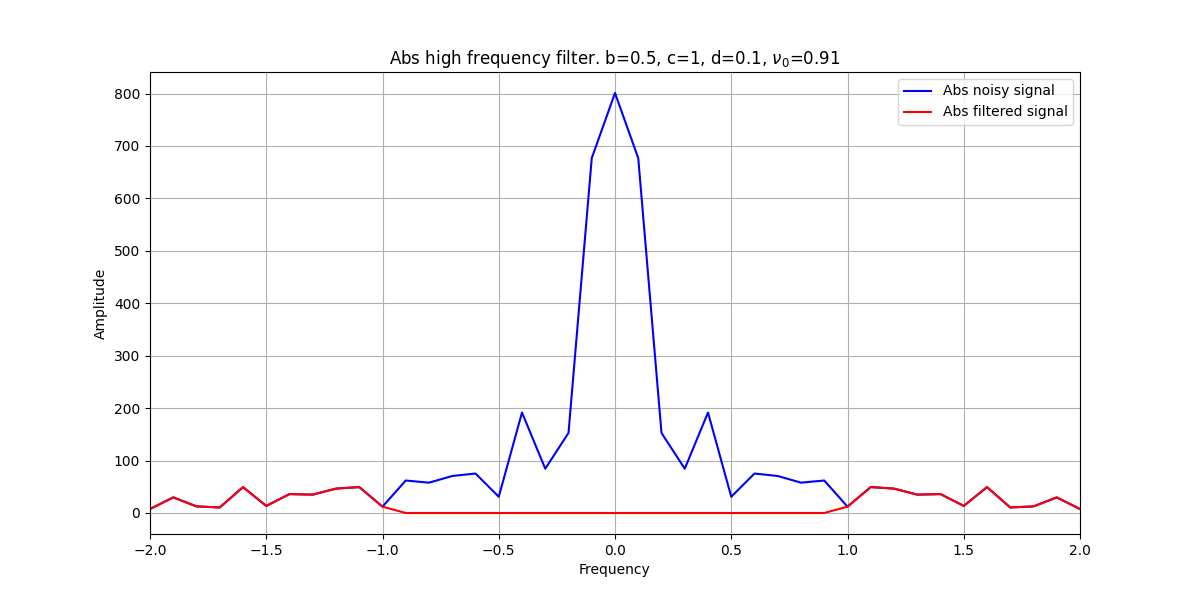
\includegraphics[scale=0.485]{9_abs_u_U_nolow.png}
        \captionsetup{skip=0pt}
        \caption{График модуля Фурье-образа исходного и фильтрованного сигналов}
        \label{fig:fig44}
    \end{figure}
    \begin{figure}[!htb]
        \centering
        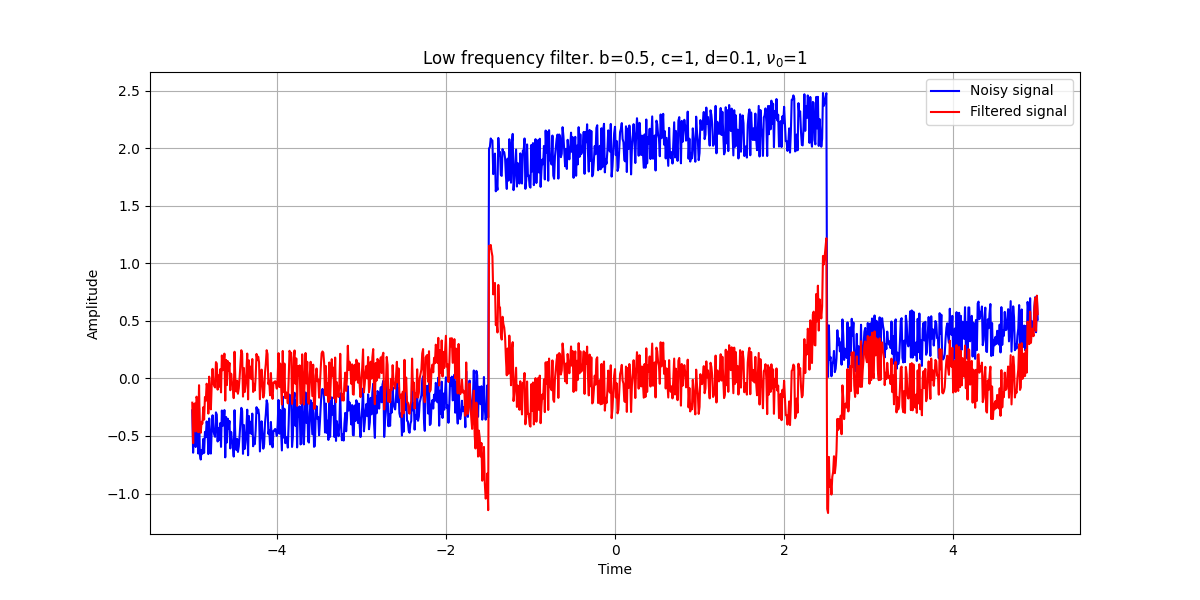
\includegraphics[scale=0.485]{10_u_flt_u_nolow.png}
        \captionsetup{skip=0pt}
        \caption{График исходного и фильтрованного сигналов}
        \label{fig:fig45}
    \end{figure}
    \begin{figure}[!htb]
        \centering
        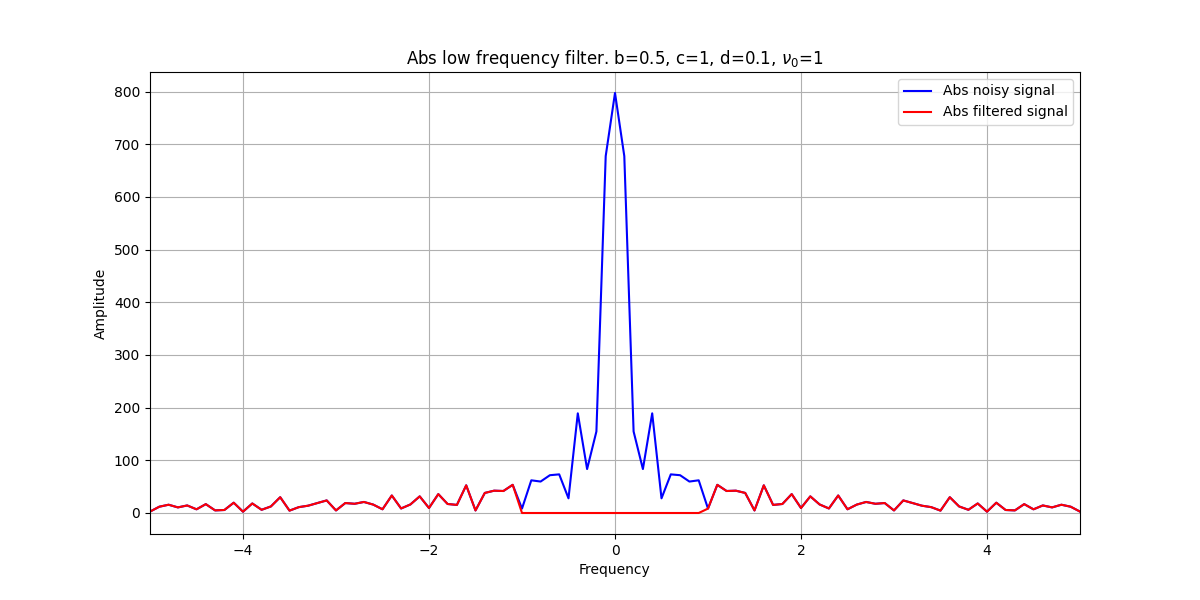
\includegraphics[scale=0.485]{10_abs_u_U_nolow.png}
        \captionsetup{skip=0pt}
        \caption{График модуля Фурье-образа исходного и фильтрованного сигналов}
        \label{fig:fig46}
    \end{figure}
    \begin{figure}[!htb]
        \centering
        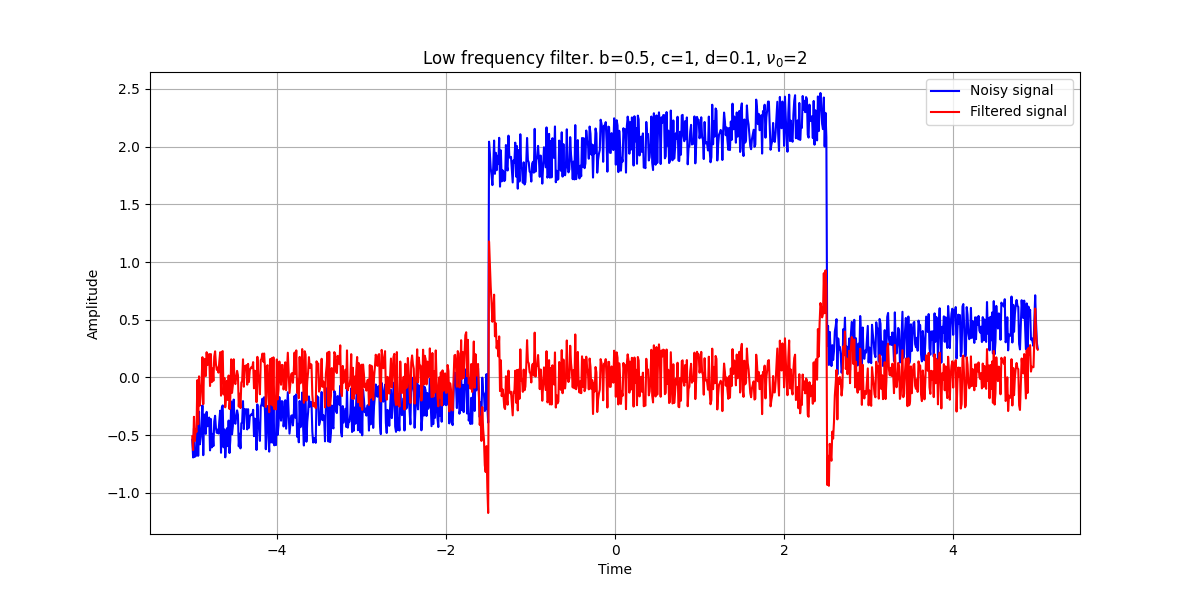
\includegraphics[scale=0.485]{11_u_flt_u_nolow.png}
        \captionsetup{skip=0pt}
        \caption{График исходного и фильтрованного сигналов}
        \label{fig:fig47}
    \end{figure}
    \begin{figure}[!htb]
        \centering
        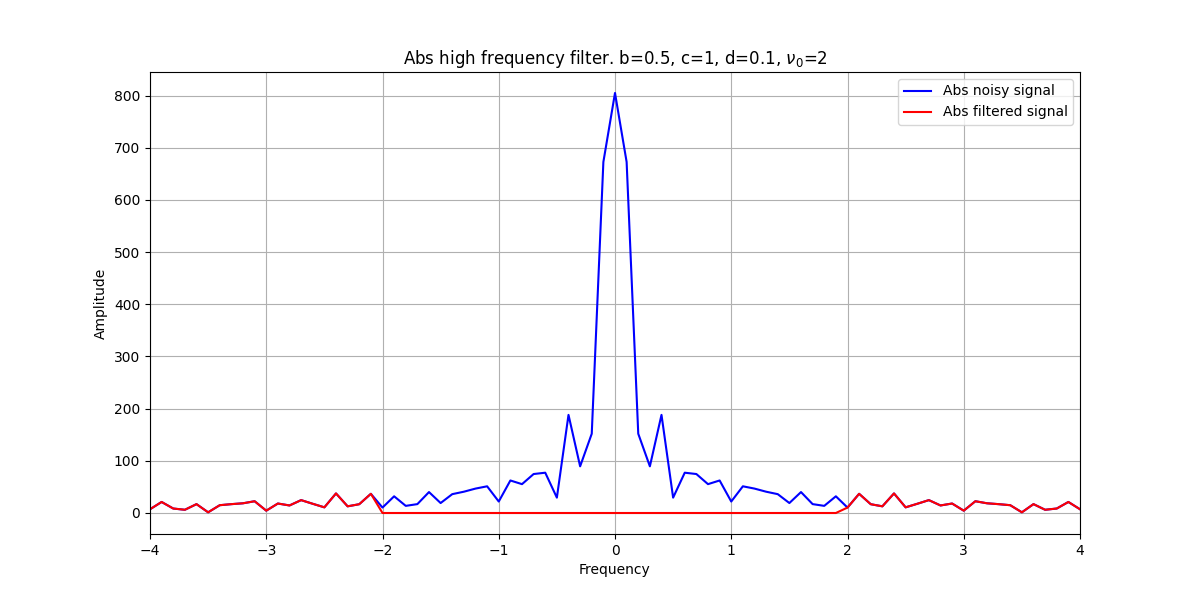
\includegraphics[scale=0.485]{11_abs_u_U_nolow.png}
        \captionsetup{skip=0pt}
        \caption{График модуля Фурье-образа исходного и фильтрованного сигналов}
        \label{fig:fig48}
    \end{figure}
    \begin{figure}[!htb]
        \centering
        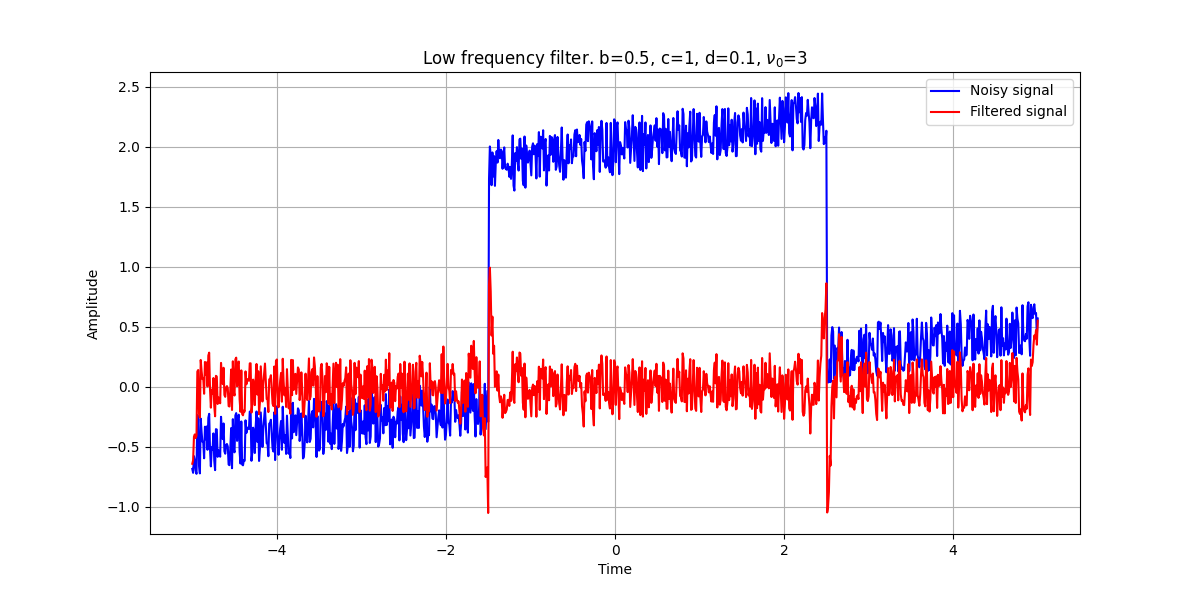
\includegraphics[scale=0.485]{12_u_flt_u_nolow.png}
        \captionsetup{skip=0pt}
        \caption{График исходного и фильтрованного сигналов}
        \label{fig:fig49}
    \end{figure}
    \begin{figure}[!htb]
        \centering
        \includegraphics[scale=0.485]{12_abs_u_U_nolow.png}
        \captionsetup{skip=0pt}
        \caption{График модуля Фурье-образа исходного и фильтрованного сигналов}
        \label{fig:fig50}
    \end{figure}
    \begin{figure}[!htb]
        \centering
        \includegraphics[scale=0.485]{13_u_flt_u_nolow.png}
        \captionsetup{skip=0pt}
        \caption{График исходного и фильтрованного сигналов}
        \label{fig:fig51}
    \end{figure}
    \begin{figure}[!htb]
        \centering
        \includegraphics[scale=0.485]{13_abs_u_U_nolow.png}
        \captionsetup{skip=0pt}
        \caption{График модуля Фурье-образа исходного и фильтрованного сигналов}
        \label{fig:fig52}
    \end{figure}
    \begin{figure}[!htb]
        \centering
        \includegraphics[scale=0.485]{14_u_flt_u_nolow.png}
        \captionsetup{skip=0pt}
        \caption{График исходного и фильтрованного сигналов}
        \label{fig:fig53}
    \end{figure}
    \begin{figure}[!htb]
        \centering
        \includegraphics[scale=0.485]{14_abs_u_U_nolow.png}
        \captionsetup{skip=0pt}
        \caption{График модуля Фурье-образа исходного и фильтрованного сигналов}
        \label{fig:fig54}
    \end{figure}
    \begin{figure}[!htb]
        \centering
        \includegraphics[scale=0.485]{15_u_flt_u_nolow.png}
        \captionsetup{skip=0pt}
        \caption{График исходного и фильтрованного сигналов}
        \label{fig:fig55}
    \end{figure}
    \begin{figure}[!htb]
        \centering
        \includegraphics[scale=0.485]{15_abs_u_U_nolow.png}
        \captionsetup{skip=0pt}
        \caption{График модуля Фурье-образа исходного и фильтрованного сигналов}
        \label{fig:fig56}
    \end{figure}
    \begin{figure}[!htb]
        \centering
        \includegraphics[scale=0.485]{16_u_flt_u_nolow.png}
        \captionsetup{skip=0pt}
        \caption{График исходного и фильтрованного сигналов}
        \label{fig:fig57}
    \end{figure}
    \begin{figure}[!htb]
        \centering
        \includegraphics[scale=0.485]{16_abs_u_U_nolow.png}
        \captionsetup{skip=0pt}
        \caption{График модуля Фурье-образа исходного и фильтрованного сигналов}
        \label{fig:fig58}
    \end{figure}
    \begin{figure}[!htb]
        \centering
        \includegraphics[scale=0.485]{17_u_flt_u_nolow.png}
        \captionsetup{skip=0pt}
        \caption{График исходного и фильтрованного сигналов}
        \label{fig:fig59}
    \end{figure}
    \begin{figure}[!htb]
        \centering
        \includegraphics[scale=0.485]{17_abs_u_U_nolow.png}
        \captionsetup{skip=0pt}
        \caption{График модуля Фурье-образа исходного и фильтрованного сигналов}
        \label{fig:fig60}
    \end{figure}
    \begin{figure}[!htb]
        \centering
        \includegraphics[scale=0.485]{18_u_flt_u_nolow.png}
        \captionsetup{skip=0pt}
        \caption{График исходного и фильтрованного сигналов}
        \label{fig:fig61}
    \end{figure}
    \begin{figure}[!htb]
        \centering
        \includegraphics[scale=0.485]{18_abs_u_U_nolow.png}
        \captionsetup{skip=0pt}
        \caption{График модуля Фурье-образа исходного и фильтрованного сигналов}
        \label{fig:fig62}
    \end{figure}
    \begin{figure}[!htb]
        \centering
        \includegraphics[scale=0.485]{19_u_flt_u_nolow.png}
        \captionsetup{skip=0pt}
        \caption{График исходного и фильтрованного сигналов}
        \label{fig:fig63}
    \end{figure}
    \begin{figure}[!htb]
        \centering
        \includegraphics[scale=0.485]{19_abs_u_U_nolow.png}
        \captionsetup{skip=0pt}
        \caption{График модуля Фурье-образа исходного и фильтрованного сигналов}
        \label{fig:fig64}
    \end{figure}
    \begin{figure}[!htb]
        \centering
        \includegraphics[scale=0.485]{20_u_flt_u_nolow.png}
        \captionsetup{skip=0pt}
        \caption{График исходного и фильтрованного сигналов}
        \label{fig:fig65}
    \end{figure}
    \begin{figure}[!htb]
        \centering
        \includegraphics[scale=0.485]{20_abs_u_U_nolow.png}
        \captionsetup{skip=0pt}
        \caption{График модуля Фурье-образа исходного и фильтрованного сигналов}
        \label{fig:fig66}
    \end{figure}
    \begin{figure}[!htb]
        \centering
        \includegraphics[scale=0.485]{21_u_flt_u_nolow.png}
        \captionsetup{skip=0pt}
        \caption{График исходного и фильтрованного сигналов}
        \label{fig:fig67}
    \end{figure}
    \begin{figure}[!htb]
        \centering
        \includegraphics[scale=0.485]{21_abs_u_U_nolow.png}
        \captionsetup{skip=0pt}
        \caption{График модуля Фурье-образа исходного и фильтрованного сигналов}
        \label{fig:fig68}
    \end{figure}


    \subsection{Убираем специфические частоты.}
    Возьмем ненулевые параметры $b,\,c,\,d$ и проделаем то же самое, что и раньше. Сначала попробуем
    обнулять некоторые диапазоны частот, потом обнулим верхние или нижние частоты, а также
    совместим различные варианты фильтрации, чтобы по возможности убрать влияние обеих компонент помехи.
    Исследуем влияние частот среза и значений параметров $b,\,c,\,d$ на вид помехи и эффективность
    фильтрации. Кроме того, отдельно рассмотрим случай для $b=0$.


    Далее будут приведены рисунки полученных графиков. На каждом графике подписаны выбранные значения $b,\,c,\,d,\,\nu_0$. 
    Также отмечена легенда -- синим цветом обозначается оригинальный сигнал, красным фильтрованный. Для первого случая будут
    добавлены два дополнительных рисунка -- графики сигнала и его Фурье-образа. Второй из двух нужен для того, чтобы выбрать
    диапазон частот, который мы будем обнулять. В ходе эксперимента с различными диапазонами был сделан вывод, что нужно попробовать
    обнулять те частоты, которые имеют пиковые амплитуды рядом с наивысшей амплитудой в точке 0. Если наивысшая амплитуда не одна, а, например,
    их две, и они находятся где-то в окресности точки 0, то обнулять будем пики частот слева от левой и справа от правой наивысших амплитуд.
    Частоты в этих диапазонах будем называть специфическими.

    
    % todo анализ
    \begin{figure}[!htb]
        \centering
        \includegraphics[scale=0.485]{1_u_nospec.png}
        \captionsetup{skip=0pt}
        \caption{График исходного сигнала}
        \label{fig:fig69}
    \end{figure}
    \begin{figure}[!htb]
        \centering
        \includegraphics[scale=0.485]{1_fft_u_nospec.png}
        \captionsetup{skip=0pt}
        \caption{График Фурье-образа исходного сигнала}
        \label{fig:fig70}
    \end{figure}
    \begin{figure}[!htb]
        \centering
        \includegraphics[scale=0.485]{1_u_flt_u_nospec.png}
        \captionsetup{skip=0pt}
        \caption{График исходного и фильтрованного сигналов}
        \label{fig:fig71}
    \end{figure}
    \begin{figure}[!htb]
        \centering
        \includegraphics[scale=0.485]{1_abs_u_U_nospec.png}
        \captionsetup{skip=0pt}
        \caption{График модуля Фурье-образа исходного и фильтрованного сигналов}
        \label{fig:fig72}
    \end{figure}
    \begin{figure}[!htb]
        \centering
        \includegraphics[scale=0.485]{1_1_u_flt_u_nospec.png}
        \captionsetup{skip=0pt}
        \caption{График исходного и фильтрованного сигналов}
        \label{fig:fig73}
    \end{figure}
    \begin{figure}[!htb]
        \centering
        \includegraphics[scale=0.485]{1_1_abs_u_U_nospec.png}
        \captionsetup{skip=0pt}
        \caption{График модуля Фурье-образа исходного и фильтрованного сигналов}
        \label{fig:fig74}
    \end{figure}
    \begin{figure}[!htb]
        \centering
        \includegraphics[scale=0.485]{1_2_u_flt_u_nospec.png}
        \captionsetup{skip=0pt}
        \caption{График исходного и фильтрованного сигналов}
        \label{fig:fig75}
    \end{figure}
    \begin{figure}[!htb]
        \centering
        \includegraphics[scale=0.485]{1_2_abs_u_U_nospec.png}
        \captionsetup{skip=0pt}
        \caption{График модуля Фурье-образа исходного и фильтрованного сигналов}
        \label{fig:fig76}
    \end{figure}
    \begin{figure}[!htb]
        \centering
        \includegraphics[scale=0.485]{2_u_flt_u_nospec.png}
        \captionsetup{skip=0pt}
        \caption{График исходного и фильтрованного сигналов}
        \label{fig:fig77}
    \end{figure}
    \begin{figure}[!htb]
        \centering
        \includegraphics[scale=0.485]{2_abs_u_U_nospec.png}
        \captionsetup{skip=0pt}
        \caption{График модуля Фурье-образа исходного и фильтрованного сигналов}
        \label{fig:fig78}
    \end{figure}
    \begin{figure}[!htb]
        \centering
        \includegraphics[scale=0.485]{2_1_u_flt_u_nospec.png}
        \captionsetup{skip=0pt}
        \caption{График исходного и фильтрованного сигналов}
        \label{fig:fig79}
    \end{figure}
    \begin{figure}[!htb]
        \centering
        \includegraphics[scale=0.485]{2_1_abs_u_U_nospec.png}
        \captionsetup{skip=0pt}
        \caption{График модуля Фурье-образа исходного и фильтрованного сигналов}
        \label{fig:fig80}
    \end{figure}
    \begin{figure}[!htb]
        \centering
        \includegraphics[scale=0.485]{2_2_u_flt_u_nospec.png}
        \captionsetup{skip=0pt}
        \caption{График исходного и фильтрованного сигналов}
        \label{fig:fig81}
    \end{figure}
    \begin{figure}[!htb]
        \centering
        \includegraphics[scale=0.485]{2_2_abs_u_U_nospec.png}
        \captionsetup{skip=0pt}
        \caption{График модуля Фурье-образа исходного и фильтрованного сигналов}
        \label{fig:fig82}
    \end{figure}
    \begin{figure}[!htb]
        \centering
        \includegraphics[scale=0.485]{3_u_flt_u_nospec.png}
        \captionsetup{skip=0pt}
        \caption{График исходного и фильтрованного сигналов}
        \label{fig:fig83}
    \end{figure}
    \begin{figure}[!htb]
        \centering
        \includegraphics[scale=0.485]{3_abs_u_U_nospec.png}
        \captionsetup{skip=0pt}
        \caption{График модуля Фурье-образа исходного и фильтрованного сигналов}
        \label{fig:fig84}
    \end{figure}
    \begin{figure}[!htb]
        \centering
        \includegraphics[scale=0.485]{4_u_flt_u_nospec.png}
        \captionsetup{skip=0pt}
        \caption{График исходного и фильтрованного сигналов}
        \label{fig:fig85}
    \end{figure}
    \begin{figure}[!htb]
        \centering
        \includegraphics[scale=0.485]{4_abs_u_U_nospec.png}
        \captionsetup{skip=0pt}
        \caption{График модуля Фурье-образа исходного и фильтрованного сигналов}
        \label{fig:fig86}
    \end{figure}
    \begin{figure}[!htb]
        \centering
        \includegraphics[scale=0.485]{4_u_flt_u_nospec_v2.png}
        \captionsetup{skip=0pt}
        \caption{График исходного и фильтрованного сигналов}
        \label{fig:fig87}
    \end{figure}
    \begin{figure}[!htb]
        \centering
        \includegraphics[scale=0.485]{4_abs_u_U_nospec_v2.png}
        \captionsetup{skip=0pt}
        \caption{График модуля Фурье-образа исходного и фильтрованного сигналов}
        \label{fig:fig88}
    \end{figure}
    \begin{figure}[!htb]
        \centering
        \includegraphics[scale=0.485]{4_u_flt_u_nospec_v3.png}
        \captionsetup{skip=0pt}
        \caption{График исходного и фильтрованного сигналов}
        \label{fig:fig89}
    \end{figure}
    \begin{figure}[!htb]
        \centering
        \includegraphics[scale=0.485]{4_abs_u_U_nospec_v3.png}
        \captionsetup{skip=0pt}
        \caption{График модуля Фурье-образа исходного и фильтрованного сигналов}
        \label{fig:fig90}
    \end{figure}
    \begin{figure}[!htb]
        \centering
        \includegraphics[scale=0.485]{4_u_flt_u_nospec_v4.png}
        \captionsetup{skip=0pt}
        \caption{График исходного и фильтрованного сигналов}
        \label{fig:fig91}
    \end{figure}
    \begin{figure}[!htb]
        \centering
        \includegraphics[scale=0.485]{4_abs_u_U_nospec_v4.png}
        \captionsetup{skip=0pt}
        \caption{График модуля Фурье-образа исходного и фильтрованного сигналов}
        \label{fig:fig92}
    \end{figure}
    \begin{figure}[!htb]
        \centering
        \includegraphics[scale=0.485]{5_u_flt_u_nospec.png}
        \captionsetup{skip=0pt}
        \caption{График исходного и фильтрованного сигналов}
        \label{fig:fig93}
    \end{figure}
    \begin{figure}[!htb]
        \centering
        \includegraphics[scale=0.485]{5_abs_u_U_nospec.png}
        \captionsetup{skip=0pt}
        \caption{График модуля Фурье-образа исходного и фильтрованного сигналов}
        \label{fig:fig94}
    \end{figure}
    \begin{figure}[!htb]
        \centering
        \includegraphics[scale=0.485]{5_1_u_flt_u_nospec.png}
        \captionsetup{skip=0pt}
        \caption{График исходного и фильтрованного сигналов}
        \label{fig:fig95}
    \end{figure}
    \begin{figure}[!htb]
        \centering
        \includegraphics[scale=0.485]{5_1_abs_u_U_nospec.png}
        \captionsetup{skip=0pt}
        \caption{График модуля Фурье-образа исходного и фильтрованного сигналов}
        \label{fig:fig96}
    \end{figure}
    \begin{figure}[!htb]
        \centering
        \includegraphics[scale=0.485]{5_2_u_flt_u_nospec.png}
        \captionsetup{skip=0pt}
        \caption{График исходного и фильтрованного сигналов}
        \label{fig:fig97}
    \end{figure}
    \begin{figure}[!htb]
        \centering
        \includegraphics[scale=0.485]{5_2_abs_u_U_nospec.png}
        \captionsetup{skip=0pt}
        \caption{График модуля Фурье-образа исходного и фильтрованного сигналов}
        \label{fig:fig98}
    \end{figure}
    \begin{figure}[!htb]
        \centering
        \includegraphics[scale=0.485]{6_u_flt_u_nospec.png}
        \captionsetup{skip=0pt}
        \caption{График исходного и фильтрованного сигналов}
        \label{fig:fig99}
    \end{figure}
    \begin{figure}[!htb]
        \centering
        \includegraphics[scale=0.485]{6_abs_u_U_nospec.png}
        \captionsetup{skip=0pt}
        \caption{График модуля Фурье-образа исходного и фильтрованного сигналов}
        \label{fig:fig100}
    \end{figure}
    \begin{figure}[!htb]
        \centering
        \includegraphics[scale=0.485]{6_1_u_flt_u_nospec.png}
        \captionsetup{skip=0pt}
        \caption{График исходного и фильтрованного сигналов}
        \label{fig:fig101}
    \end{figure}
    \begin{figure}[!htb]
        \centering
        \includegraphics[scale=0.485]{6_1_abs_u_U_nospec.png}
        \captionsetup{skip=0pt}
        \caption{График модуля Фурье-образа исходного и фильтрованного сигналов}
        \label{fig:fig102}
    \end{figure}
    \begin{figure}[!htb]
        \centering
        \includegraphics[scale=0.485]{6_2_u_flt_u_nospec.png}
        \captionsetup{skip=0pt}
        \caption{График исходного и фильтрованного сигналов}
        \label{fig:fig103}
    \end{figure}
    \begin{figure}[!htb]
        \centering
        \includegraphics[scale=0.485]{6_2_abs_u_U_nospec.png}
        \captionsetup{skip=0pt}
        \caption{График модуля Фурье-образа исходного и фильтрованного сигналов}
        \label{fig:fig104}
    \end{figure}
    \begin{figure}[!htb]
        \centering
        \includegraphics[scale=0.485]{7_u_flt_u_nospec.png}
        \captionsetup{skip=0pt}
        \caption{График исходного и фильтрованного сигналов}
        \label{fig:fig105}
    \end{figure}
    \begin{figure}[!htb]
        \centering
        \includegraphics[scale=0.485]{7_abs_u_U_nospec.png}
        \captionsetup{skip=0pt}
        \caption{График модуля Фурье-образа исходного и фильтрованного сигналов}
        \label{fig:fig106}
    \end{figure}
    \begin{figure}[!htb]
        \centering
        \includegraphics[scale=0.485]{7_1_u_flt_u_nospec.png}
        \captionsetup{skip=0pt}
        \caption{График исходного и фильтрованного сигналов}
        \label{fig:fig107}
    \end{figure}
    \begin{figure}[!htb]
        \centering
        \includegraphics[scale=0.485]{7_1_abs_u_U_nospec.png}
        \captionsetup{skip=0pt}
        \caption{График модуля Фурье-образа исходного и фильтрованного сигналов}
        \label{fig:fig108}
    \end{figure}
    \begin{figure}[!htb]
        \centering
        \includegraphics[scale=0.485]{7_2_u_flt_u_nospec.png}
        \captionsetup{skip=0pt}
        \caption{График исходного и фильтрованного сигналов}
        \label{fig:fig109}
    \end{figure}
    \begin{figure}[!htb]
        \centering
        \includegraphics[scale=0.485]{7_2_abs_u_U_nospec.png}
        \captionsetup{skip=0pt}
        \caption{График модуля Фурье-образа исходного и фильтрованного сигналов}
        \label{fig:fig110}
    \end{figure}


    \section{Задание 2. Фильтрация звука.}
    В данном задании необходимо убрать шумы из записи голоса в файле MUHA.wav так, чтобы остался только голос. 
    При прослушивании записи голос слышно не очень хорошо, так как присутствует громкий гул. Построим графики
    исходного сигнала аудиозаписи и его Фурье-образа. Определим по второму графику, какие частоты могут создавать
    шумы. Так как гул громкий, нам необходимо вырезать самые высокие частоты из аудиозаписи. Такие частоты мы можем
    наблюдать примерно в диапазоне $[-300,300]$ Гц. Чтобы вырезать эти частоты, потребуется фильтр нижних частот, который
    мы рассматривали в задании 1. После применения фильтра построим сравнительный график исходного и фильтрованного
    сигналов аудиозаписи. Можем наблюдать, насколько чище стал сигнал -- оставшиеся амплитуды являются голосом, который 
    нам нужен. Это легко понять исходя из того, что между каждым возрастанием амплитуд есть интервал с падением амплитуд, 
    где они находится в некоторой окресности нуля -- это паузы в предложении, которое говорит человек на записи. Также построим
    сравнительный график модуля исходного и фильтрованного сигналов аудиозаписи. На нем мы видим, что мы успешно вырезали
    самые высокие частоты, которые соответствовали громкому гулу. Теперь послушаем аудиозапись filtered\_{MUHA}.wav, которая 
    оставлена на этом \href{https://drive.google.com/drive/folders/1AuXIiKRWvXFOtJqV3uqPzC494zZ7vCrd?usp=sharing}{гугл-диске}, 
    и убедимся в том, что все посторонние шумы пропали. На записи голос слышно хорошо, однако остался некоторый звуковой эффект 
    фейзер. Избавиться от него мне удалось только обрезав частоты в диапазоне $[-22050, -1000]$ и $[1000, 22050]$ Гц, однако
    голос сильно потерял в качестве. Прослушать этот вариант можно на том же \href{https://drive.google.com/drive/folders/1AuXIiKRWvXFOtJqV3uqPzC494zZ7vCrd?usp=sharing}{гугл-диске},
    файл выложен под названием filtered\_{MUHA}\_{2}.wav.


    Далее представлены рисунки с графиками, о которых говорилось в предыдущем абзаце. Синим цветом обозначен исходный сигнал,
    красным -- фильтрованный. Также представлены графики для фильтрованной аудиозаписи filtered\_{MUHA}\_{2}.wav. Стоит заметить,
    что на рисунке \ref{fig:fig116} видно, как окресность нуля стала меньше по сравнению с рисунком \ref{fig:fig113}, то есть в 
    подобных диапазонах амплитуды частот уменьшились.


    \begin{figure}[!htb]
        \centering
        \includegraphics[scale=0.485]{noisy_audio.png}
        \captionsetup{skip=0pt}
        \caption{График исходного сигнала аудиозаписи}
        \label{fig:fig111}
    \end{figure}
    \begin{figure}[!htb]
        \centering
        \includegraphics[scale=0.485]{U_audio.png}
        \captionsetup{skip=0pt}
        \caption{График Фурье-образа исходного сигнала аудиозаписи}
        \label{fig:fig112}
    \end{figure}
    \begin{figure}[!htb]
        \centering
        \includegraphics[scale=0.485]{u_flt_u_audio.png}
        \captionsetup{skip=0pt}
        \caption{График исходного и фильтрованного сигналов аудиозаписи}
        \label{fig:fig113}
    \end{figure}
    \begin{figure}[!htb]
        \centering
        \includegraphics[scale=0.485]{abs_u_U_audio.png}
        \captionsetup{skip=0pt}
        \caption{График модуля Фурье-образа исходного и фильтрованного сигналов аудиозаписи}
        \label{fig:fig114}
    \end{figure}
    \begin{figure}[!htb]
        \centering
        \includegraphics[scale=0.485]{u_flt_u_audio_v2.png}
        \captionsetup{skip=0pt}
        \caption{График исходного и фильтрованного сигналов аудиозаписи}
        \label{fig:fig115}
    \end{figure}
    \begin{figure}[!htb]
        \centering
        \includegraphics[scale=0.485]{abs_u_U_audio_v2.png}
        \captionsetup{skip=0pt}
        \caption{График модуля Фурье-образа исходного и фильтрованного сигналов аудиозаписи}
        \label{fig:fig116}
    \end{figure}


    \section{Листинги программных реализаций}
    В этой секции будут рассмотрены программные реализации, которые использовались по ходу выполнения лабораторной работы.
\end{document}